%%%%%%%%%%%%%%%%%%%%%%%%%%%%%%%%%%%%%%%%%%%%%%%%%%%%%%%%%%%%%%%%%%%%%%%
%% $Id: report.tex,v 1.5 2005/02/09 21:06:42 lindstrm Exp $
%%%%%%%%%%%%%%%%%%%%%%%%%%%%%%%%%%%%%%%%%%%%%%%%%%%%%%%%%%%%%%%%%%%%%%%
%% costhesis usage example
%% modified and added to by GQMJr
%%%%%%%%%%%%%%%%%%%%%%%%%%%%%%%%%%%%%%%%%%%%%%%%%%%%%%%%%%%%%%%%%%%%%%%
%
% The costhesis package accepts the following options
%
%   Document types:
%     msc               - Master Thesis
%     bsc		- Kandidate Thesis
%
%   Layout options:
%
%   Other options:
%     blank             - Removes pagenumbers and headers from empty pages
%     blankmsg          - Prints a message of intent on empty pages
%     scheader          - Typeset headers in SMALL CAPS shape (default)
%     slheader          - Typeset headers in slanted shape 
%
%
%
%

\documentclass[12pt,a4paper,twoside,openright]{book}
%%\documentclass[12pt,a4paper,twoside,openright]{memoir}

\usepackage[msc,blankmsg]{costhesis}
%\usepackage[T1]{fontenc}
%%\usepackage{pslatex}
\renewcommand{\rmdefault}{ptm} 
\usepackage{mathptmx}
\usepackage[scaled=.90]{helvet}
\usepackage{courier}
%
\usepackage{bookmark}
\usepackage{subfigure}
\usepackage{tabularx}

%%----------------------------------------------------------------------------
%%   pcap2tex stuff
%%----------------------------------------------------------------------------
 \usepackage[dvipsnames*,svgnames]{xcolor} %% For extended colors
 \usepackage{tikz}
 \usetikzlibrary{arrows,decorations.pathmorphing,backgrounds,fit,positioning,calc,shapes}
% \usepackage{pgfmath}	% --math engine
%%----------------------------------------------------------------------------
\usepackage[latin1]{inputenc}
%\usepackage[utf8]{inputenc} % inputenc allows the user to input accented characters directly from the keyboard
\usepackage[french,swedish,english]{babel}
\usepackage{rotating}		 %% For text rotating
\usepackage{array}			 %% For table wrapping
\usepackage{graphicx}	 %% Support for images
\usepackage{float}			 %% Suppor for more flexible floating box positioning
\usepackage{color}           %% Support for colour 
\usepackage{mdwlist}
\usepackage{setspace}    %% For fine-grained control over line spacing
\usepackage{listings}		%% For source code listing
\usepackage{bytefield}    %% For packet drawings
\usepackage{tabularx}		%% For simple table stretching
\usepackage{multirow}	%% Support for multirow colums in tables
\usepackage{dcolumn}	%% Support for decimal point alignment in tables
\usepackage{url}	%% Support for breaking URLs
\usepackage[perpage,para,symbol]{footmisc} %% use symbols to ``number'' footnotes and reset which symbol is used first on each page

\usepackage{todonotes}
%%\usepackage{pygmentize}  %% required to use minted -- see python-pygments - Pygments is a Syntax Highlighting Package written in Python
%\usepackage{minted}		%% For source code highlighting
%\usemintedstyle{borland}

\usepackage{hyperref}		
\usepackage[all]{hypcap}	 %% Prevents an issue related to hyperref and caption linking
%% setup hyperref to use the darkblue color on links
\hypersetup{colorlinks,breaklinks,
            linkcolor=darkblue,urlcolor=darkblue,
            anchorcolor=darkblue,citecolor=darkblue}


%% Some definitions of used colors
\definecolor{darkblue}{rgb}{0.0,0.0,0.3} %% define a color called darkblue
\definecolor{darkred}{rgb}{0.4,0.0,0.0}
\definecolor{red}{rgb}{0.7,0.0,0.0}
\definecolor{lightgrey}{rgb}{0.8,0.8,0.8} 
\definecolor{grey}{rgb}{0.6,0.6,0.6}
\definecolor{darkgrey}{rgb}{0.4,0.4,0.4}
%% Reduce hyphenation as much as possible
\hyphenpenalty=15000 
\tolerance=1000

%% useful redefinitions to use with tables
\newcommand{\rr}{\raggedright} %% raggedright command redefinition
\newcommand{\rl}{\raggedleft} %% raggedleft command redefinition
\newcommand{\tn}{\tabularnewline} %% tabularnewline command redefinition

%% definition of new command for bytefield package
\newcommand{\colorbitbox}[3]{%
	\rlap{\bitbox{#2}{\color{#1}\rule{\width}{\height}}}%
	\bitbox{#2}{#3}}

%% command to ease switching to red color text
\newcommand{\red}{\color{red}}
%%redefinition of paragraph command to insert a breakline after it
\makeatletter
\renewcommand\paragraph{\@startsection{paragraph}{4}{\z@}%
  {-3.25ex\@plus -1ex \@minus -.2ex}%
  {1.5ex \@plus .2ex}%
  {\normalfont\normalsize\bfseries}}
\makeatother

%%redefinition of subparagraph command to insert a breakline after it
\makeatletter
\renewcommand\subparagraph{\@startsection{subparagraph}{5}{\z@}%
  {-3.25ex\@plus -1ex \@minus -.2ex}%
  {1.5ex \@plus .2ex}%
  {\normalfont\normalsize\bfseries}}
\makeatother

\setcounter{tocdepth}{2}	%% 3 depth levels in TOC
\setcounter{secnumdepth}{5} %% 3 sectioning levels. WARNING: command \mainmatter resets this field to its default value!!!
%%%%%%%%%%%%%%%%%%%%%%%%%%%%%%%%%%%%%%%%%%%%%%%%%%%%%%%%%%%%%%%%%%%%
%% End of preamble
%%%%%%%%%%%%%%%%%%%%%%%%%%%%%%%%%%%%%%%%%%%%%%%%%%%%%%%%%%%%%%%%%%%%

\iauthor{Alexandre Kohen}
\ititle{Unified Communications with Lync 2013}
\isubtitle{}
\idate{2013}{October}{1}
\examinername{Prof. G. Q. Maguire Jr.}

\setlength{\headheight}{15pt}
\begin{document}

\frontmatter
\selectlanguage{english}
\begin{abstract}
\label{sec:abstract}
\setcounter{page}{1}
Unified Communications solutions bring together several communication modes, technologies, and applications in order to answer businesses' and individuals' growing need for simpler, faster, and more effective communications means.
Although many hardware-based products allow the integration of telephony within a computer network environment, telephony features of software-based unified communications solutions are seldom used, which limits their effectiveness or requires another solution to be used jointly.

This master's thesis project aims to demonstrate that unified communications solutions based on Microsoft Lync Server 2013 can effectively address a wide variety of business scenarios, including a traditional telephony system replacement.

The first part of this master's thesis introduces background knowledge about unified communications and associated technologies, as well as the different components of the selected unified communication solution.

The case study presented in this thesis is the first large-scale Lync 2013 deployment with a complete telephony offering in France. The presentation follows the complete deployment process, starting from the analysis of the client's needs to the solution design, construction, and validation.

This project demonstrated the suitability of Lync 2013 as a telephony system replacement. However, the transition from a classic telephony solution to a unified communications solution can be a technical challenge. An essential step in making this transition successful was to take the users' needs into account. It was also essential to accompany these users throughout the transition.

\end{abstract}
%%\clearpage
\selectlanguage{swedish}
%%\chapter*{Sammanfattning}
\begin{abstract}
\label{sec:swedish_abstract}

Samordnad kommunikation (engelska: unified communications) l�sningar \linebreak[4]sammanf�ra flera kommunikationss�tt,
teknik och till�mpningar f�r att besvara f�retags och individers
v�xande behovet av enklare, snabbare och mer effektivt kommunikationsmedel.
�ven m�nga h�rdvara-baserade produkter till�ter \linebreak[4]integration av telefoni
inom ett datorn�tverk milj�, telefoni funktioner \linebreak[4]mjukvarubaserad
Samordnad kommunikation-l�sningar anv�nds s�llan, vilket begr�nsar deras effektivitet
eller kr�ver en annan l�sning f�r att anv�ndas gemensamt.
Detta examensarbete syftar till att visa att samordnad kommunikation
l�sningar baserade p� Microsoft Lync Server 2013 kan effektivt ta itu med en
m�ngd olika scenarier. Den f�rsta delen av detta examensarbete introducerar
bakgrundskunskap om samordnad kommunikation och tillh�rande teknologier
liksom de olika komponenterna i den valda samordnad kommunikation
l�sning.

Fallstudien som presenteras i denna avhandling �r den f�rsta storskaliga Lync 2013
utplacering med en komplett telefoni erbjuder i Frankrike. Den presentationen
f�ljer hela implementeringsprocessen, fr�n analys av kundens
kraven till utformning, konstruktion, och validering.
Detta projekt visade \linebreak[4]tillf�rlitligheten i Lync 2013 som telefoni ers�ttning
men intyga att �ven �verg�ngen fr�n en klassisk telefoni l�sning p� ett
samordnad kommunikation-l�sning kan vara en teknisk utmaning, ta anv�ndarnas
behov i beaktande och medf�ljande anv�ndare genom �verg�ngen �r kritisk.
\end{abstract}

\selectlanguage{french}
%%\chapter*{Sammanfattning}
\begin{abstract}
\label{sec:french_abstract}

Les solutions de communications unifi�es rassemblent diff�rents modes de \linebreak[4] communications, technologies, et applications pour r�pondre aux besoin croissant des entreprises et individus de m�thodes de communications plus simples, rapides et efficaces. Bien que de nombreuses solutions mat�rielles permettent l'int�gration de la t�l�phonie � un r�seau informatique, les fonctions de t�l�phonie des solutions logicielles sont rarement utilis�es, ce qui limite leur efficacit� ou n�cessite l'utilisation conjointe d'autres solutions.

Ce projet a pour but de d�montrer l'efficacit� des solutions de communications unifi�es bas�es sur Microsoft Lync 2013 � r�pondre � une grande vari�t� de besoins professionels, dont le remplacement d'un syst�me de t�l�phonie traditionnel.

La premi�re partie de ce m�moire introduit les notions n�cessaires sur les communications unifi�es et les technologies associ�es, ainsi que les diff�rents composants de la solution de communications unifi�es choisie.

L'�tude de cas pr�sent�e d�crit le premier d�ploiement majeur de Lync Server 2013 comportant une offre de t�l�phonie compl�te en France, et suit le processus de d�ploiement complet, de l'analyse des besoins client � la validation du projet, en passant par la conception, la construction et le test.

Ce projet d�montre l'aptitude de Lync en temps que syst�me de t�l�phonie complet. Cependant la transition d'un syst�me traditionnel � une solution de communications unifi�es peut pr�senter des d�fis techniques, et il est essentiel de prendre en compte les besoins utilisateurs ainsi que de les accompagner durant la transition.

\end{abstract}

\selectlanguage{english}
\begin{acknowledgements}
ACK
\end{acknowledgements}

\selectlanguage{english}
\tableofcontents

\listoffigures

\listoftables


% \begin{notations}
% \end{notations}

\renewcommand\abbreviationsname{List of Acronyms and Abbreviations}
\begin{abbreviations}
\label{list-of-acronyms-and-abbreviations}


\begin{basedescript}{\desclabelstyle{\pushlabel}\desclabelwidth{10em}}

\item[AD] Active Directory
\item[CA] certification authorities

\item[OS] operating system

\item[PBX] private branch exchange
\item[PSTN] public switched telephone network
\item[QoS] Quality of Service
\item[RBAC] role-based access control
\item[SPIT] Spam over Internet Telephony
\item[SSL] Secure Sockets Layer
\item[TLS]  Transport Layer Security

\item[UM] unified messaging

\item[VoIP] voice over IP
\item[WAN]  wide area network
\item[WLAN] wireless local area network
\end{basedescript}
\end{abbreviations}

\mainmatter
\setcounter{secnumdepth}{3}


\chapter{Introduction}
%Topic introduction (size, mobility, devices, infrastructure costs, other...)
%Tech introduction
%Problem statement


%Overview, Problem description, Aim and goals, Structure
% IP-based Multimedia Subsystem
%Growing business needs (for communications and business productivity/process)and increased technical potential => continual evolution of solutions =>/ Since the 2000s, the demand for unified communications steadily increased, until being
% UC now necessary for most global companies. Mature products, but still rely on PSTN solutions for voice.
\paragraph{}
The evolution of technology and business needs allowed previously existing means of communications to converge into unified communications (UC) solutions, which allow companies to be more efficient and productive. UC solutions were originally designed by telephony or routing equipment manufacturers, while consumers used hardware-based telephony features in UC solutions; therefore, the telephony features of software-based UC solutions are rarely used, for example only 11\% of Microsoft Lync deployment is used for telephony\cite{elizabeth_harrin_unified_2013}.

The release of Microsoft Lync 2013 was aimed mostly at improving upon the Microsoft Lync Server 2010 features in order to deliver a more robust telephony solution. At the time of the start of this thesis project there were few large scale Lync 2013 telephony enabled deployments.

Therefore, the goal of this thesis project was to demonstrate Lync 2013 telephony features in an actual, large scale deployment. This particular deployment was challenging, as it was the first large scale Lync 2013 complete telephony replacement in France, the project had a tight schedule, and many features depended on other vendors' solutions. This last aspect was particularly unusual for a project conducted through Microsoft Consulting Services.

%\section{Background}
%\section{Overview}
\section{Thesis outline}
This report is divided into 5 chapters.
Chapter \ref{chapter_background} presents unified communications, along with relevant protocols and concepts. This chapter should help people new to unified communications or computer networks understand the context of unified communications and the challenges of this project.
Chapter \ref{chapter_ms_UC} describes the different components of the specific Microsoft unified communications solution that was used for this project. This chapter is recommended for readers unfamiliar with Microsoft server solutions.
Chapter \ref{chapter_case} documents the deployment design, construction, and test process.
The final chapter summarizes the conclusions, suggests future work, and gives some reflections on the social, ethical, and economic aspects of this thesis project.




%\section{Research methodology}
%No, here you would say that you are going to use (1) an experimental method to verify a hypothesis or (2) you are going to use some other research methodology in your thesis project (then explain what this method is).


\chapter{Background}\label{chapter_background}
\paragraph{}
\textit{This chapter presents the background required for a good understanding of this thesis.}

\textit{Readers unacquainted with the concepts of unified communications and cloud computing are advised to read the first and second sections, in which these concepts are briefly introduced and contextualized.}

\textit{Sections 2.3, 2.4, and 2.5 should be relevant for all readers as they present some existing software solutions, the underlying technologies and protocols, as well as the legal background which any solution has to be consistent with.}


\section{Unified Communications}
\label{background_uc}

Unified communications solutions can be described as the integration and\linebreak[4]management of various communications services, both real-time and asynchronous, such as instant messaging, telephony, SMS, presence information, video conferencing, or email; just to name a few. This integrated set of services should be accessible from a variety of devices, with the objective of increasing productivity and ease of use.

Unified communications is not a single technology nor a single software solution, but encompasses all solutions providing suitable functionality, while providing a simplified and unified user experience~\cite{fikry_unified_2012, riemer_unified_2009, pleasant_what_2008}.


\subsection{History}
Unified communications exploits the convergence of information technology and telecommunications as components to create a solution, which requires that these components must inter-operate seamlessly~\cite{riemer_unified_2009}. In order to understand the process leading to the appearance of unified communications in their current form, we must consider the evolution of telecommunications, IT, and business expectations.


\subsubsection{Business expectations}
Over the last few years, business needs have evolved. Companies now need to operate over wide geographical areas, thus business tools for mobile employees routinely include laptops, mobile phones, and tablets. Similarly when employees are at fixed locations, they increasingly have personal computers and other devices connect to local area networks or wireless local area networks (WLANs).

Business requirements have driven a continuously increasing need for mobility and real-time access to information, to enable employees to remain productive while on the move, to allow teams to remain functional even while their members are at different physical sites, and to provide employees with permanent access to up-to-date information in order to make better decisions\cite{mcknight_mobile_2011}.


\subsubsection{Unified Messaging}
The combination of the existing email and voice mail into an unified interface was achieved during the 1990s by various partnerships between software and telecommunications companies. The goal of unified messaging (UM) was to provide a single access point for the various asynchronous communications services, such as fax, email, and voice mail\cite{pleasant_what_2008}. These solutions include ``Telephony One Stop" created by Lotus and AT\&T in 1995 or ``Octel Unified Messaging" created by Microsoft and Octel in 1997\cite{parker_short_2009}.

These solutions gradually improved over time with the addition of new functions, such as instant messaging, presence signaling, advanced message management, and cross-media messaging. These functions now form the core of modern unified communications solutions.


\subsubsection{Integration with business telephony systems}

The advances in computing power and device capabilities allowed private branch exchange (PBX) manufacturers to integrate UM solutions and new features into their telephony equipment in order to meet business expectations\cite{parker_short_2009}. These features often included advanced voice mail and call forwarding management, ``find me/follow me" features allowing users to reached, desktop notification of incoming calls, and voice management\cite{pleasant_what_2008}.

\subsubsection{Voice over Internet Protocol}
With the constant increase in network capacity, it became very attractive to use a portion of this capacity to carry voice communications, due to its potential to reduce costs by taking advantage of the simplified voice over IP (VoIP) architecture. Although packet speech was first demonstrated in 1974 on the ARPANET\cite{gray_1974_2005}, the first widespread consumer VoIP application was InternetPhone, developed in 1995 by Vocaltech, Inc. which allowed its users to use their computers, microphones, and speakers to communicate with each other over the Internet\cite{hallock_brief_2004}.

VoIP became widespread in the following years, and is now very popular for both the consumer market, with solutions such as Skype, and the professional market, with solutions such as Microsoft Lync, Google Voice, and Asterisk. Lync will be further studied in this thesis project.


\subsubsection{Unified Communications}
The current state of unified communications solutions is due to the convergence of the increased needs of the companies; the core functionality provided by the existing UM solutions; and the enhanced communications solutions first introduced within PBX systems, but for which pure software counterparts now exist.

These communications systems are complemented by business productivity solutions (word processing, spreadsheets, presentation software, etc.), which were developed to fulfill the needs of various professionals.

The combination of unified communications and business solutions have attracted a lot of attention from companies, and have now established themselves as an essential tool for medium to large-sized business. The adoption of these solutions is seen in the exploding market for unified communications solutions\cite{infonetics_research_infonetics:_2012}. Additionally, Asterisk and other solutions have been expanding these types of services into small offices and even homes.


\subsection{Components}

\paragraph{}
As noted earlier, unified communications solutions are not defined by a single piece of software, hence they are always composed of different components which interacting together to provide the desired end user experience. This section lists the main categories of these components. However, not all of these components are included in every solution, nor are all of them available in every device. The actual set of components depends upon the specific implementation and the specific requirements that an implementation is targeting. Some solutions may also include additional components that do not fit into these categories\cite{ahamed_comprehensive_2008}.

\subsubsection{Call control}
Call control components allow the user to have unified control over their telephony communications. For example, information about incoming calls may be displayed on the user's current display (a computer screen for example) and the user can accept or reject calls via their computers. Users can also initiate a call from their computer, but utilize their cellular or desktop phone to participate in the actual call.

\subsubsection{Multimodal communication}
Multimodal communication allows users to reach others via an unified system, while using various means to do so.
For example, users can add a new user to their contacts list by name,  e-mail address, IM account, etc. then send this user an instant message, before establishing a voice communication session. Subsequently the participants in this session might start a shared screen activity.

\subsubsection{Voice over IP}
Often wrongly confused with unified communications, VoIP can play a crucial role in many unified communications solutions. The term VoIP is used to designate a form of communication which allows voice (and other multimedia)  communication sessions to be carried over a computer network instead of using a telephone network.

VoIP services can be interconnected with the public switched telephone network (PSTN), thus allow communications between people connected to a computer network using hardware or software VoIP clients, and people using the telephony network using cellphones or fixed digital /analog phones\cite{desantis_understanding_2008}.

\subsubsection{Presence}
Presence information is mainly used to access the availability of users for participation in a communication session. For example, the most common and simple presence application is a contacts list (often called a "buddy list") indicating whether contacts are online, offline, or unavailable for communication. In unified communications systems, presence is often at the center of the solution, hence the systems offers a variety of information, such as availability, localization, skills, or currently supported means of communication for a session\cite{peternel_using_2008}\cite{schulzrinne_simple_2006}. 

\subsubsection{Mobility}
Mobility refers to the ability to maintain a session in spite of any changes in location (terminal mobility), role change (personal mobility), or changes in which devices are used (service mobility)\cite{wang_mobility_2001}.

\subsubsection{Instant Messaging}
The ability to communicate in real-time using text messages can be a very simple, yet powerful way to communicate quickly and effectively. Therefore real time text messaging (often called ``instant communication") is a critical component of all unified communications solutions. Although most users are already familiar with consumer instant messaging solutions, enterprise systems have higher security and privacy requirements, so dedicated solutions must be used\cite{pleasant_what_2008}.

\subsubsection{Unified Messaging}
Unified messaging (UM) components are designed to provide users with a single interface for various communications systems, such as email, SMS/MMS, voice mail, and instant messaging\cite{banner_understanding_2010}.
\begin{figure}[h!]
	\centering
	\includegraphics[width=0.8\textwidth]{Schemas/um.pdf}
	\caption[Typical communications system]{Typical communications system}
	\label{fig:um_typical}
\end{figure}

\begin{figure}[h!]
	\centering
	\includegraphics[width=0.8\textwidth, page=2]{Schemas/um.pdf}
	\caption[Client-based UM]{Typical communications system}
	\label{fig:um_client}
\end{figure}

\begin{figure}[h!]
	\centering
	\includegraphics[width=0.8\textwidth, page=3]{Schemas/um.pdf}
	\caption{Server-based UM}
	\label{fig:um_server}
\end{figure}

\clearpage

\subsubsection{Speech access and personal assistant}
Personal assistants allow users to access enhanced functionality from low level devices, such as basic phones. Examples of this functionality include using a speech recognition and synthesis based interface to manage a calendar, meetings, or out of office status\cite{pleasant_what_2008}.


\subsubsection{Collaboration tools}
Collaboration tools enable enhanced communications between many users, such as audio and video conferencing, screen sharing, whiteboarding, and document sharing tools\cite{riemer_unified_2009}.

\subsubsection{Business process integration}
Integration with business processes and workflow applications is a key to reducing ``human latency" , thus increasing efficiency. Unified communications solutions integrated with a business process can, for example, reduce the delay between tasks by facilitating the notification of available and relevant personnel in the case of workflow problems\cite{pleasant_what_2008}.

\subsection{Devices}

\paragraph{}
To ensure that users can have sufficient mobility while retaining access to the communication system, unified communications solutions must be able to support a very wide range of devices, in many different situations. These devices include:

\begin{description}

\item[Computers]
Desktops and laptops have become one of the main access points to modern communications systems, due to their ability to provide the user with a rich experience. Computers are usually able to access all the functions of the unified communications solution. They can also simulate other devices functions, for example, software used to duplicate a hardware phone's functionality is called a "softphone".

\item[Cellphones]
Cellphones (or cellular phones) are essential access points for unified communications systems, as almost all business users always carry a cellphone with them, which makes the user reachable as long as they are within a compatible network's coverage area. Today these cellular telephony systems enable users to be always potentially reachable, and these systems can provide various functionality, depending on the phone's features.

Today smartphones with internet access can be used for almost all services.

\item[Tablets and netbooks]
Tablets and netbooks can be considered either as computers or smartphones, depending on their features. They usually provide the same functionality as computers if they have the appropriate hardware, and they can also be used as a smartphone if they have GSM, 3G, LTE, wireless local area network (WLAN), or similar access.

\item[Phones]
Although not as mobile as cellular phones, or able to provide the same rich experience as a computer, other types of phones are also very common in unified communications architectures for different reasons. Users are used to using a landline phone, and may prefer to use a phone handset to make calls rather than a computer headset. Some users may also not have a computer at their working location.

While limited, these phones can still provide some advanced features, beside voice calls, due to speech assistants (for example).

Moreover, there are also IP phones, connecting directly to the local area network that can provide advanced features.\cite{desantis_understanding_2008}



\item[Web clients]
Web clients can allow users to access communications services from any device able to run a compatible browser, without installing software on the device, which enables the use of public computers while on the go. For some examples of softphone functionality provided this way see \cite{arumugam_mathivanan_minisip_2012}.

\item[Other devices]
There are also other dedicated devices used in UC solutions, for example, dedicated conferencing devices allow users to hold a meeting in a conference room while streaming the video and audio from the room to remote users participating in the meeting.

\end{description}


\subsection{Vendors}
\paragraph{}
There are many different UC solutions currently on the market, most of them offering the same core features, but sometimes with very different design philosophies and technical choices. This section describes the Avaya, Cisco, and Microsoft offerings, as they are current leaders in UC solutions.

\begin{description}
\item[Avaya]
is a business collaboration and communications solutions provider and comes from a strong telephony background, as it was originally part of Lucent Technologies and AT\&T and has 12\% of the world PBX market\cite{elizabeth_harrin_unified_2013}. Avaya is one of the leading unified communications vendors, with telephony-based products, such as the Avaya Aura, or their IP Deskphones families\cite{_avaya_2012}.


\item[Cisco]
is the leading provider of routers, switches, WLAN, and telepresence equipment, and is a leading UC provider with its Unified Communications Manager\cite{elizabeth_harrin_unified_2013, _cisco_????}.


\item[Microsoft]
is originally a software company, and provides software-based UC solutions. Unlike Avaya and Cisco, Microsoft does not manufacture phones or other telephony devices and instead certifies other vendors' devices for use with Lync, such as Aastra's IP Phones or Polycom's meeting rooms devices
\cite{microsoft_technet_phones_2013}.
\end{description}


\subsection{Conclusions}
\paragraph{}
UC can be very interesting for organizations, as it can help reduce communications costs by replacing some (or all) of the PSTN traffic by VoIP  traffic over a data network, which is typically a lot cheaper - especially for long distance calls. It can also help companies increase efficiency by enabling employee mobility, and facilitating communications, both within the company, and with partners or clients. UC solutions also reduce the time required to find or contact people relevant to each situation, and can help optimize business processes, which can make employees' lives easier, while enabling the employee to be more efficient and productive. SIP-based communications can also provide increased security against interception due to traffic encryption\cite{carrara_security_2005} which makes UC all the more attractive to businesses.

Due to its added value, UC is becoming an essential business requirement and the market for UC solutions is currently rapidly expanding.
However, UC poses new challenges, as the transfer of communications from the PSTN to a computer network leads to new issues, such as the need for continuous, high bandwidth, low latency Internet connectivity and the need to supply the electrical power needed by and consumed by the required equipment. A thesis that address this power consumption is \cite{talaganov_green_2012}.

Moreover, unified communications solutions also raise new security, confidentiality, and compliance issues, such as the need for users without PSTN access to be able to contact emergency services, and the risk of Spam over Internet Telephony (SPIT) that can be induced by VoIP communications\cite{desantis_understanding_2008}.

%Market share
%New opportunities/possibilities
%Now essential business requirement
%New challenges

\section{Protocols}
Although there is no standard UC protocol, some basic protocols are used in almost all UC solutions. 

\subsection{Internet Protocol (IP)}
\paragraph{Function}
The Internet Protocol is the main communication protocol used in computer networks and is responsible for routing data packets between hosts. Each packet has two sections, the header which contains information about the packet (such as the source address, destination address, and type), and the payload (which is the actual data to be delivered to the destination)\cite{rfc791}.

\paragraph{IP Address}
The IP Address is used when forwarding IP packets to their destination. In most cases, an IP address identifies a single computer's interface on a network.
There are currently two active versions of the Internet Protocol, IPv4 with 32 bit addresses, such as 172.16.254.1\cite{rfc791}, and IPv6 with 128 bit addresses, such as 2001:db8:85a3:0:0:8a2e:370:7334. IPv6 was created to remedy to the current shortage of IPv4 addresses\cite{rfc2460}.

Each subnet is allocated with a range of IP addresses which can be allocated to devices within this subnet. To indicate a subnet address, the notation $address/mask$ is used, where $mask$ is the number of leading bits in the subnet address.
For example, the IPv4 block 172.16.254.0/24 represents the addresses from 172.16.254.0 to 172.16.254.255.

\paragraph{Usage}
Unlike in circuit-switched networks, IP networks are packet-switched and use dynamic routing: each node along a path makes a local routing decision for each packet. Most of the routing in IP networks is done by dedicated equipments, called routers, which forward incoming packets according to a routing table.

The design of IP networks has several consequences:
\begin{itemize}
\item There is no delivery guarantee or error correction. Endpoints must check the message integrity.
\item A message can be several packets long and not all of these packets have to take to same path to reach the destination.
\item In case of link or node failure occurring only between two packets, the message can still be transmitted.
\end{itemize}


\subsection{Domain Name System (DNS)}
\paragraph{}
The major use of the Domain Name System (DNS) is to translate an domain name to an IP address. This IP address can then be used to contact the desired host. While DNS resolution uses IP packets, the process of IP routing and DNS resolution are completely unrelated.

DNS is a hierarchical and distributed system, with each sub-domain belonging to a higher level domain recursively up to a root level. Each DNS server can delegate authority over a sub-domain to another DNS server. A zone is the set of domains and sub-domains over which a name server has authority.

In a domain name, labels are separated by dots and ordered by hierarchy, with the top-level domain being on the right, and the lowest level domain on the left (just after the host's name within this lowest level domain).
A Fully Qualified Domain Name (FQDN) is a domain name that includes its full hierarchy, up to the root domain.

When resolving a DNS address to an IP address, clients will usually contact a recursive DNS resolver. This resolver will perform queries as necessary to each level's authoritative server, in order to resolve the name into an IP address.

DNS resolvers usually exploit caching to save previous and intermediate queries' results, which can avoid the need for a complete DNS look-up for each request.  Details of the performance of today's DNS system can be found in \cite{bentahar_dns_2013}.



\subsection{Transport Layer Security}
\paragraph{}
The Transport Layer Security (TLS) protocol provides security for transport layers such as TCP. TLS is commonly used to provide security to HTTP\cite{rfc5246, rescorla_ssl_2000}. TLS is a successor of the Secure Sockets Layer (SSL) protocol.

TLS uses client and server certificates (asymmetric keys) to generate a common session key which is used to encrypt the data between the client and the server.

STARTTLS is a protocol extension that allows upgrading a plain text connection to an TLS encrypted connection on the same port instead of using a dedicated port for encrypted connections.


\subsection{Lightweight Directory Access Protocol (LDAP)}
The Lightweight Directory Access Protocol (LDAP) is an Internet protocol for accessing distributed directory services. This is a standard protocol that allows multiple applications to access an LDAP-compliant server to retrieve information such as contacts, but also certificates, printers, services, or any other information that can be stored in a directory
\cite{rfc4510}.

\subsection{Kerberos}

Kerberos is a protocol allowing authentication of users on a network using asymmetric cryptography and the use of tickets. The PKINIT extension for Kerberos adds the use of a smartcard or USB authenticator to the authentication, and is often used in Microsoft Windows environments to provide strong\linebreak[4]authentication\cite{rfc4120,rfc4556}.

\subsection{Session Initiation Protocol (SIP)}

The Session Initiation Protocol (SIP) has been developed and standardized by the Internet Engineering Task Force (IETF) and is used to control real-time multimedia communication sessions over IP networks. This protocol is widely used in VoIP to create, modify or terminate sessions\cite{rfc3261}.

The H.323 recommendation by the ITU-T also defines the H.225.0 and H.245 protocols, which are also used in some VoIP solutions\cite{dalgic_comparison_1999}.


\subsection{Extensible Messaging and Presence Protocol (XMPP)}
The Extensible Messaging and Presence Protocol (XMPP) allows the exchange of messages based on XML over IP networks. XMPP is used in many applications, such as Jabber or Google Talk, for instant messaging, presence information, or contact list\cite{rfc6120}.

\section{Other useful concepts}
The following concepts are not specific to UC solutions, but play a significant role in realizing a modern UC system.


\subsection{Virtualization}
\paragraph{}
Virtualization refers to the set of techniques used to separate a process from its physical operating environment.
There are multiple reasons for virtualization depending on the type of virtualization, such as hardware efficiency, application availability, or faster development cycles
\cite{alan_murphy_virtualization_2008}.

The most common type of virtualization is operating system virtualization, which allows a host machine to execute several virtual machines. There are multiple advantages to this type of virtualization over physical computers:
\begin{itemize}
\item A single computer can host multiple low usage virtual machines, so there is less computing power wasted when one virtual machine is not used;
\item More flexibility, as the virtual machine resource usage can be modified in real time;
\item Faster deployment;
\item Simpler migration or failover; and
\item Allows the creation of secure or test environments separated from the host computer environment.
\end{itemize}

Moreover, virtualization is a necessary component for most cloud computing offerings.

\subsection{Cloud Computing}\label{background_cloud}
\paragraph{}
Cloud computing is a term describing a variety of computing concepts related to distributed computing and the transfer of part of the computing infrastructure responsibilities to a service provider. Due to the ubiquitous nature of UC solutions, cloud computing is an important component of many UC offerings.

Cloud computing is usually divided into different categories, depending on how responsibilities are separated\cite{peter_mell_nist_2011}:

\begin{description}
\item[Software as a Service (SaaS)]
In this service model, a service provider assumes complete responsibility over an application and grants usage rights to clients usually for a monthly or yearly fee.
This can cause greatly reduced IT costs for the clients by removing the need for maintaining hardware or software, and simplifies scalability.
Microsoft Office 365 or Google Apps are examples of SaaS.

\item[Platform as a Service (PaaS)] 
In this model, the provider offers a computing platform on which the client can run its applications. This allows the client to focus on its applications.
Web hosting is an example of PaaS. 

\item[Infrastructure as a Service (IaaS)] 
In a IaaS model, the providers offers access to computers. Usually this model relies heavily on virtual machines to provide the required service levels (better availability, scaling, and backup). Unlike in PaaS, the client has full access to the operating system and can use the computers for any use.
IaaS offers the client more control, better scalability, and security with a lower upfront investment. 
Microsoft Windows Azure and Amazon Elastic Compute Cloud (EC2) are examples of IaaS providers.

\end{description}



\subsection{Quality of Service (QoS)}
\paragraph{}
Quality of Service (QoS) refers to the quality of service which the end user perceives (or an application receives). QoS can also refer to the set of techniques used to enable traffic to cross the network while satisfying certain quality parameters. The relevant quality parameters to guarantee to ensure a good service differ depending on the type of traffic considered, but the most common parameters are: bandwidth, latency, packet loss, and jitter.

The goal of guaranteeing QoS is that users of an application transmitting packets over the network will experience good service. Best-effort handling of packets, which is the default operating mode of the network, simply forwards packets in their order of arrival without offering any QoS guarantees. This delivery method is sufficient when the traffic is low compared to the network capacity and when the service level requirements are low. However, with higher service requirements or insufficient network capacity, this approach leads to degraded service during peaks in the network traffic.

A simple approach would be to over provision resources, so that the network capacity is always greater than the requested usage. However, this would lead to a costly network with most on the resources left unused, except during what many only be brief usage peaks.

PSTN calls use circuit switching to guarantee the service level during a call; hence when a call is to be initiated, resources are allocated for the call, and cannot be used by any other calls until this call has terminated, which guarantees a constant service level. If there are not enough resources available, then the call cannot be established.

The postal service is also a best-effort type network, as letters are transmitted as they are received by the postal service, with additional delays if there is a sudden burst of letters sent. However, there are different rates for different types of letters, with higher rates guaranteeing faster delivery.

\paragraph{IP Networks}
There are two main protocols to support Quality of Service in IP Networks, Differentiated Services (DiffServ)\cite{rfc2474} and Integrated Services (IntServ)\cite{rfc1633}.


\subsection{Public Key Cryptography}
A public key algorithm relies on the use of asymmetric keys to encrypt and decrypt messages. Unlike in conventional (or symmetric) cryptography, the keys used to encrypt and decrypt the message are different. This allows the secure exchange of messages, with a decreased risk that the common secret used to encrypt the message is intercepted, and to generate cryptographic signatures. A Public Key Infrastructure (PKI) refers to a set of physical or logical components used to create, store, distribute and verify digital certificates\cite{stallings_cryptography_2014}.

\section{Legal}\label{background_legal}

In France, there are many laws and rules applicable to UC, but no specific legislation and very little case-law. Therefore the resulting legal background for UC is complex, but cannot be ignored as it can affect UC solution deployment and operations.

\subsection{Privacy}
There can be privacy concerns over the content of the communications held through a UC solution. In France, there is no specific law, but different general laws apply, such as the law on the privacy of letters, and on telecommunications exchanges. According to these laws, it's illegal for someone who is not a recipient of a message to prevent or delay its delivery, tamper, read, or diffuse its content\cite{_atteinte_????,_loi_????,_loi_????-1}. However this applies only to communications identified as personal\cite{_cour_????}. Professional communications have different legislation, depending on the company.


\subsection{Archiving and compliance}
UC solutions must also take archiving and compliance with regulation into account. For example, some documents, such as contracts or commercial correspondence must be kept for up to 10 years\cite{_code_????-1,_code_????-2}, international companies may have to respect regulation such as the Sarbanes-Oxley\cite{_sarbanes-oxley_????} or local law\cite{_loi_2005}, which imposes a higher degree of security, and specific scope, duration, and format for archiving.


\subsection{Safety}
Telephony solutions must implement regional standards, such as E911, to allow access to emergency services\cite{_voip_????}.

\subsection{Other}
Other legislation might have unexpected impact on UC solutions. For example, regulation on the usage of the electromagnetic frequencies limits the strength of signals using the 2.4GHz and 5GHz frequencies, which are used for WiFI. Moreover, the frequencies between 5.25GHz and 5.725GHz are also used for military and meteo radars, which have priority over WiFi emissions\cite{arcep_reseaux_????}.


\section{Related Work}

Although there is little available documentation on Lync 2013, a lot of work has already been done on Lync 2010 and other UC solutions.

\subsection{Lync deployment}
There are multiple sources of documentation for planning and deploying Microsoft Lync 2010, such as Microsoft IT's Deploying Lync Server 2010 whitepaper\cite{microsoft_it_showcase_deploying_2011}, and Microsoft TechNet\cite{microsoft_technet_microsoft_2013}.


\subsection{Disaster Recovery and Business Continuity Planning in Action: Japan 2011}
This article, published by Microsoft IT in July 2011, follows the March 2011 earthquake in Japan and its impact on the Lync 2010 infrastructure, as well as the disaster recovery processes used and the lessons learned\cite{microsoft_it_showcase_disaster_2011}.

\chapter{Microsoft Unified Communication Solution}\label{chapter_ms_UC}
\paragraph{}
\textit{This chapter presents the Microsoft unified communications solution that is the focus of this master's thesis project. This solution is made up of different closely interconnected software solutions, and each section will present a separate piece of this software. The sections are ordered by integration order, with each piece of software using functions from the previous ones.}
\textit{The complete chapter is essential reading to achieve a good understanding of this master's thesis. The sections on Lync 2013 and Active Directory are particularly relevant.}

\section{Windows Server}
Microsoft Windows Server is the operating system (OS) for servers running in a Microsoft Windows environment, hence every server-side software solution used in this project is running on top of Microsoft Windows Server. Relevant details of this OS will be given below.

\subsection{OS for servers}
\paragraph{}
The OS's task is to manage the computer's resources and to provide resources and services to applications.

The latest version of Microsoft Windows Server is currently Windows Server 2012. For this thesis project, only Windows Server 2008 R2 (Datacenter edition) and Windows Server 2012 (Standard or Datacenter editions) were used.


\subsection{Features}
\paragraph{}
Windows Server 2008 R2 and Windows Server 2012 are respectively the server version of Windows 7 and Windows 8, therefore they share many of their features with their client counterpart. However, as a server version of the OS, they have some additional features, with the biggest difference being their focus on high availability, scalability, higher security, and ease of administration. Some of the most relevant features of these OSs for this project are:

\paragraph{Virtualization}
The integrated virtualization functions of Windows Server 2008 R2 and 2012 allow simple configuration and administration of virtual machines (VMs). This facilitates the creation of lab environments to prototype and test a complete architecture on a single machine or the administration of a production environment where many lightly loaded VMs are run on the same physical server. The integrated VM manager in Windows Server 2008 R2 and 2012 is called Hyper-V.

\paragraph{Active Directory}
Windows Server has native support for Active Directory. A given server can be assigned any Active Directory role without requiring any additional software installation. Further details of active directory can be found in section 3.2.

\paragraph{High Availability}
Some of the features of Windows Server 2008 R2 and 2012 help to achieve the high availability requirements of UC applications. Among these features are functions to allow administrators to create failover clusters (which allows unreachable servers to be automatically replaced), to use a virtual storage pool to ensure high data availability, and new virtualization tools for quick VM backups or restores without stopping running services.

\paragraph{PowerShell}
Windows PowerShell 3.0 is integrated with Windows Server 2012 and Windows Server 2008 R2 SP1. PowerShell provides a task automation framework. PowerShell consists of a command-line shell interface and an associated scripting language that allows administrative tasks to be performed on local or remote systems, using "cmdlets" which are specialized .Net classes. Unlike UNIX's shell scripting languages, interactions in PowerShell are object-based, so each command returns a .Net object that can be used by subsequent commands. This allows a programmer to quickly create powerful scripts for task automation.


\subsection{Administration tools}
\paragraph{}
There are multiple tools available to administer a Windows server. The most common ones are listed here.


\paragraph{Server Manager}
The Server Manager is a graphical interface run from the server's desktop. It allows administrators to easily monitor and manage servers in a domain. It provides simple tools for monitoring events and server performance, and managing roles for a whole server group without the need to connect directly to each server.

\begin{figure}[h!]
	\centering
	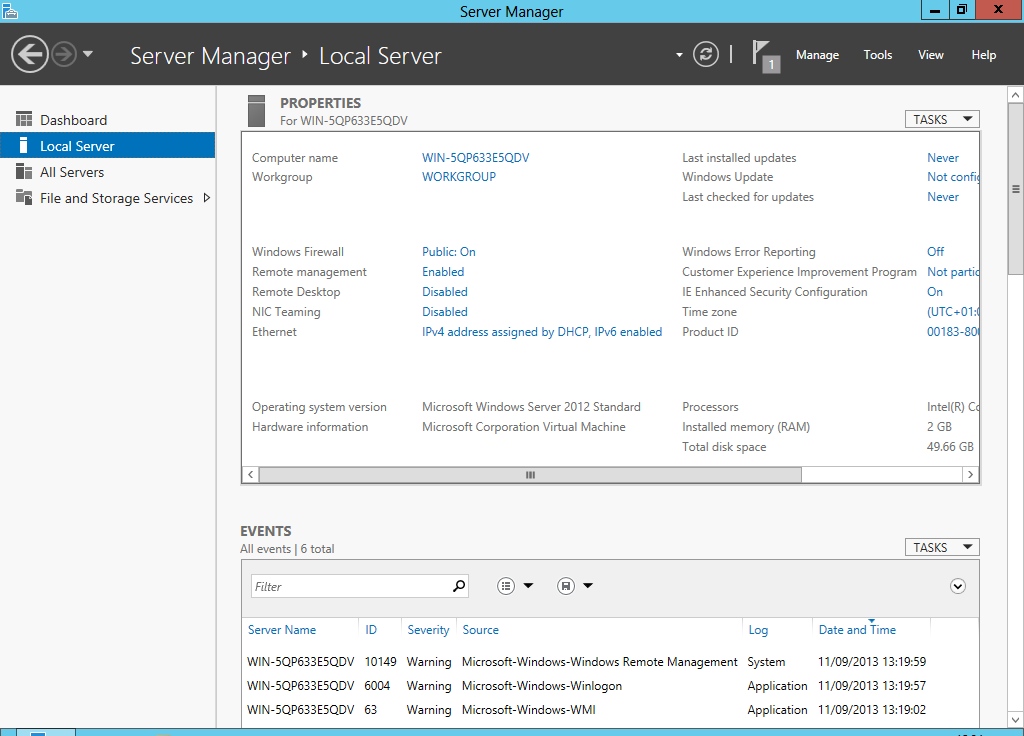
\includegraphics[width=0.8\textwidth]{Schemas/servermanager.png}
	\caption{Windows Server 2012 Server Manager}
	\label{fig:ws_sm}
\end{figure}

\paragraph{Remote Desktop Connection}
A Windows Server can also be managed remotely, via a remote Desktop Connection, which allows the administrator to remotely access a server's Desktop interface.

\paragraph{Microsoft Management Console}
The Microsoft Management Console can be used as a graphical interface for configuring and monitoring servers. The console can be customized with various snap-ins, with each snap-in providing some specific functionality.

\paragraph{PowerShell}
The PowerShell interface can be used to manage servers without using a graphical interface.
\missingfigure{screencaps/RDC/MMC/PS?}


\section{Active Directory}

Active Directory (AD) is the central repository for identities in a Microsoft environment.

\subsection{Directory Services}
\paragraph{}
AD is Microsoft's LDAP compliant directory service. AD's main function is to provide a central source for identification and authentication for computers running one of Microsoft's OSs when this computer is connected to a network. AD is able to maintain a list resources for a managed network, such as user accounts, computers, printers, shared folders, apply security or administrative policies, distribute software upgrades, and allow controlled access to network resources.

AD plays a central role in almost all of Microsoft software solutions, as it provides a lot of the basic functionality required by other software\cite{desmond_active_2008}.


\subsection{Roles}
\paragraph{}
An AD architecture is composed of multiple roles, each role providing a separate functionality. A single server can have one or many roles, and each role can be assigned to multiple servers. Only the AD Domain Services role is required to be assigned to at least one computer in any given AD architecture, all of the other roles are optional.\cite[p. 5-7]{holme_self-paced_2011}

\subsubsection{Active Directory Domain Services (AD DS)}
The central role of any AD architecture is to provide a central repository for identity management, as well as the identification and authentication services.

\subsubsection{Active Directory Lightweight Domain Services (AD LDS)}
AD LDS is used to provide a duplicate of the directory store for use by network applications. AD LDS can also be used as a more secure alternative to an AD Domain Services server in low security networks.

\subsubsection{Active Directory Certificate Services (AD CS)}
The AD CS role can be used to create a public key infrastructure by issuing digital certificates binding an identity to a certificate. A private key associated with a certificate can be used for authentication. AD Certificate Services is not always limited to a local network and can be used to provide services to external communities.

\subsubsection{Active Directory Rights Management Services (AD RMS)}
Although AD Domain Services servers can determine whether documents on the network can be accessed, they cannot control how documents are used by the identities that are allowed to access them. The AD Rights Management Services can ensure the integrity of data by enforcing usage policies for documents.

\subsubsection{Active Directory Federation Services (AD FS)}
AD FS allows the AD architecture to span different organizations or platforms, so each organization can maintain its own directory service while allowing some resources to be shared.


\subsection{Components}
\paragraph{}
Some components are necessary to describe an AD architecture.

\subsubsection{Domain Controller (DC)}
A server responsible for the AD DS role is called a Domain Controller. It provides a Kerberos Key Distribution Center authentication service, as well as other AD services\cite[p. 9]{holme_self-paced_2011}.


\subsubsection{Logical divisions of the directory service}
The smallest logical division is a domain. Each domain requires at least one domain controller, with each domain controller containing all the information about the domain's identities. A collection of domains in a contiguous DNS namespace is called a tree. Finally, the set of all the domains forms an AD forest, which is the security boundary of the directory service. The first domain in a forest is called the root domain\cite[p. 9]{holme_self-paced_2011}.

\subsubsection{Sites}
An AD site represents a portion of the enterprise within which there is high data rate and high capacity connectivity. Such a site is a boundary for replication and service usage\cite[p. 11]{holme_self-paced_2011}.

\subsubsection{Organizational Unit (OU)}
An organizational unit is a container for active directory objects, such as computers, users, or groups. An OU can contain other OUs to create a hierarchical organization. OUs are the main tool for sorting objects and selecting the scope of security or administrative policies\cite[p. 11]{holme_self-paced_2011}.

\subsubsection{Single Sign-On (SSO)}
Single Sign-On (SSO) allows a user to enter its credential only once when using multiple independent software systems. AD is often used to provide SSO to the various services a company employee might have to access, based on their AD identity, so the user only has to log into Windows to be logged into other services (such as an e-mail client or a web application), even if they are provided by another company (with the use of AD FS).

\subsubsection{Group Policy}
Group Policies are used to administer a large number of domain-joined client computers remotely. A Group Policy Object (GPO) is created by an administrator to define a behavior, linked to users, and synchronized between the AD DCs before being pushed to the client computers. Each client computer applies the different GPOs and resolves potential conflicts before enforcing the resulting configuration.


\subsection{Conclusion}
AD is a basic and critical service of a Windows based IT architecture. Since AD provides identification, authentication, and access control to the computers attached to a network, it needs to meet high availability, security, and functionality requirements.
This requires different techniques to be used, such as server redundancy, load balancing, failover systems, security protocols, and data \linebreak[4]replication techniques.


\section{Exchange}

Exchange is Microsoft's mail server that has been in development for 19 years, and encompasses more than 21 million lines of code.
The Microsoft client-side software to access Exchange services is Microsoft Outlook.

\subsection{Mail Solution}
\paragraph{}
 Exchange provides email services and requires an existing AD infrastructure to run, as it extends AD identities to create mailboxes, calendars, and contacts lists\cite[Ch. 1]{redmond_microsoft_2010}.
The latest versions of these software solutions are Microsoft Exchange 2013 and Microsoft Outlook 2013.

\subsection{Outlook 2013}
\paragraph{}
Outlook 2013 is the client-side software associated with Exchange 2013, but it can also be used as a standalone application. Its most common use is as an email application, but it can also be used for calendar, tasks, and contacts management, RSS reader, and taking notes. Thus Outlook 2013 can be used as a personal information manager.

\paragraph{}
Outlook is also available as a web application called Outlook Web App (OWA), which is used to provide remote users access to their mailbox, contacts, and calendar.

\missingfigure{Outlook2013 screencaps}

\subsection{Exchange 2013}
\paragraph{}
Exchange 2013 is the server side software of the mail solution.


\subsubsection{Active Directory}
Of all of Microsoft's applications, Exchange makes the most extensive use of AD. 
Exchange extends the AD Schema by adding new objects and adding attributes to existing objects, such as email addresses for users.
Exchange stores this information in every AD DC in the forest (for schema updates and configuration settings), and in the domain for mail-enabled user identity updates\cite[Ch. 1]{redmond_microsoft_2010}.

\subsubsection{Server Roles}
Exchange 2013 reduced the number of roles from five in Exchange 2010 down to two: the Client Access Server role and the Mailbox role. The Client Access Server is the server used by a client for authentication and redirection to the user's active mailbox server. The mailbox server stores the mailbox data. Each user's mailbox can be replicated on multiple mailbox servers, with one of them being modified directly by the user (called the active mailbox), while the others are passive copies, used in case of failure of the active mailbox server. The active mailbox server can be different for each user\cite[Ch. 1]{redmond_microsoft_2010}.

\subsubsection{Administration}
Exchange 2013 can be administered with graphical user interface (GUI) tools, such as Microsoft Management Console (MMC) snap-ins, but there are also new PowerShell 3.0 cmdlets to create scripts and automate tasks, as well as the web based Exchange Administrator Central that allows an administrator to configure the Exchange 2013 architecture from any browser\cite[Ch. 3\&5]{redmond_microsoft_2010}.

\missingfigure{Exchange admin tool}



\section{SharePoint}

SharePoint 2013 is a collaboration solution, which uses server software to provide users with collaboration tools through a web interface
\cite[Ch. 1]{husman_beginning_2010}.
SharePoint's most visible aspect is web portals, which can be used to access documents, regroup information, or access SharePoint functionality.
SharePoint can be used to create public or private web portals, such as a company's public website, or a department, team, or personal web site. Websites can be created using the desktop application SharePoint Designer 2013.
These portals can be used to create a company intranet (which is accessible only from the company's internal network), an extranet (which is available only to company employees or partners even if they are outside the company's offices), or a public website, available to all
\cite[Ch. 1]{husman_beginning_2010}.


These web portals can be used to store and share any kind of data. Moreover, Microsoft Office integration within SharePoint allows users to quickly open and save documents to or from a SharePoint site, retrieve a previous version of a document, protect documents, co-author a document in real time, synchronize contacts, or integrate Microsoft Access applications in SharePoint.

SharePoint can also be used to search for documents and information on the company's intranet. This enables any employee to use SharePoint's search engine to quickly find data among all the documents he or she has access to.

SharePoint integrates tools for document management according to various compliance standards, such as Sarbanes-Oxley (SOX) and ISO-9000
\cite[Ch. 1]{husman_beginning_2010}.



\section{Lync}

Lync is the real-time communications component of Microsoft's UC solution. Lync is composed of two different pieces of software: the Lync Server and the Lync client. This solution provides instant messaging, presence, VoIP, and conferencing functionality to users, as well as providing telephony features with the Enterprise Voice option\cite{winters_mastering_2012}.

\subsection{Client-side software}

To communicate using a Lync infrastructure, users must use one of the Lync client-side software options (i.e., client applications). Some of the characteristics and features of these clients are described in the following paragraphs.

\subsubsection{Clients}
All Lync client functionality is accessible through a client application, which can be either a desktop client (installed on the client computer), a mobile client (installed via the phone's application market), a Lync Phone (a dedicated device on which Lync is running), or a web-based client (which can be accessed from any networked computer with a supported browser\cite{microsoft_technet_lync_2013-1}). The web based client can be especially useful when inviting external partners to a meeting or to enable employees to use Lync while on the move\cite[Ch. 1.1]{winters_mastering_2012}.

\subsubsection{Contacts}
The default main screen of the Lync client is the user's contacts list, that displays this user's list of contacts, sorted by configurable groups. This list displays, for each contact: their name, picture, availability status, location, and a note.

The user can search for contacts by name or skills through the search box. Results will be displayed as contacts in the contact list, along with their role or company (if they are external contacts) and their relevant skills, in the case of a search by skill(s). Contacts can be added to groups and assigned a confidentiality level, to determine what information is available to this contact.

The user can also display the contact card for each contact. This contact card lists messaging options, contact information (such as address or phone number) and their organization information (such as their chain of managers, from their manager to the company's CEO, people with the same manager, or their collaborators). The search and contact card make it easy to find the correct person or persons quickly, enabling users to find available persons with the appropriate skills
\cite[Ch. 1.1]{winters_mastering_2012}.

\missingfigure{Contact list/search/contact card}

\subsubsection{Presence}
The Lync client can be used to access presence information of contacts within the company or within federated organizations. The contact's status is the first form of presence information. This presence information can be set manually or automatically to one of: available, away, busy, do not disturb, be right back, in a conference/call, or offline. This allows people to know how to contact the person, and when they might get an answer. This status also changes how messages will be delivered, for example, an incoming instant message will play an audio notification if the user's status is set to available, a visual notification if the person is busy, or no notification if the person should not be disturbed.

Users can also leave a note, which will be displayed under their name for all contacts, which allows for more explanation on the reasons for their absence or useful information, such as "I'm in a day-long meeting, please contact XXX if you need help today".

The user's location can also be set. When in a new location, the user can enter a name for the location. This location name will be displayed under the user's name every time they log on in the future from this same location\cite[Ch. 1.1]{winters_mastering_2012}.


\subsubsection{Instant messaging}
Instant messaging conversations can be started by double clicking on a contact name in the contacts list. Messages will be sent to the recipient's current device (computer, phone, or browser application), or delivered to them when they next connect to the Lync server. Depending on the user's  status, the recipient will get different notifications of the incoming message. The user can reply to or ignore the message. Participants in an instant messaging discussion can invite other people to join the conversation, or add voice, video, whiteboard, presentations, or other activities to the conversation. After leaving the conversation, all of the messages are recorded, and a list of previous conversations is available under the Conversation tab of the main screen.

\missingfigure{Conversation screen/list}

\subsubsection{VoIP and Enterprise Voice}
The Lync client can be used for voice communications, either by adding voice to a text conversation, or by starting a voice conversation from the contact list or a contact card. If both parties have VoIP support, then the communication is established using VoIP. This is usually the case between Lync Desktop and web clients, or other federated desktop clients, such as Skype.

If the recipient cannot be reached via VoIP, for example because they are not on a computer network, then Lync with Enterprise Voice can establish a communication session over the PSTN.
Lync Enterprise Voice users can access various telephony services, such as call forwarding, visual voicemail, device switching, enhanced emergency services, or call delegation
\cite[Ch. 1.1]{winters_mastering_2012}.

\subsubsection{Video conferencing and collaboration}
Lync also supports video conversations, and conferencing. While conferencing, users can use various media, such as text, voice, video, screen sharing, presentations, or whiteboards. They can also conduct polls and record the conversation. Users can also co-edit documents using Sharepoint during a meeting
\cite[Ch. 1.1]{winters_mastering_2012}.

\begin{figure}[h!]
	\centering
	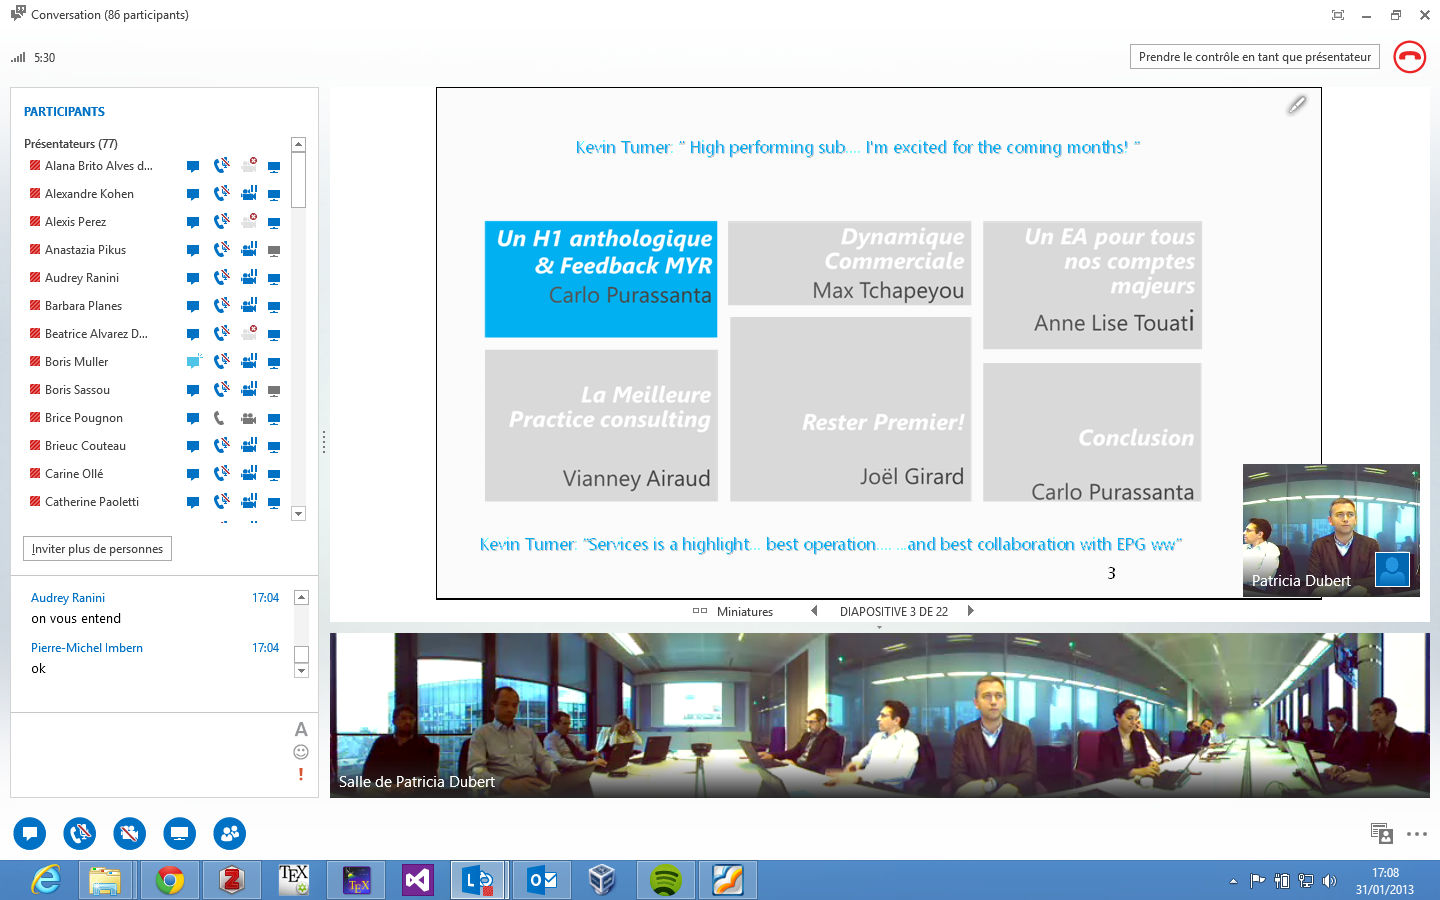
\includegraphics[width=0.8\textwidth]{Schemas/lync.png}
	\caption{Conference with Lync 2013}
	\label{fig:lync_conferencing}
\end{figure}

\subsubsection{Outlook integration}
Lync is closely integrated with Outlook and many features require both to be fully available.

For example, contact information is shared between Outlook and Lync (so users can see presence information while in Outlook) or manage contacts from both applications. Moreover, Lync archives are stored in Outlook and searchable as emails, and voicemails can be accessed from both Lync and Outlook.

Users can schedule meetings from Lync or Outlook, and add to an email a link that can be used to join a Lync meeting. Lync will also use the user's Outlook calendar to automatically update the user's presence information according to their daily schedule
\cite{winters_mastering_2012}.


\subsection{Lync Server 2013}

Lync Server 2013 is the main server-side software used to create a Lync infrastructure\cite[Ch. 1.2]{microsoft_technet_lync_2013-2,winters_mastering_2012}.
.

\subsubsection{Roles}
Each server running Lync Server runs one or more server roles. A server role is a defined set of Lync Server functionalities provided by that server.

\begin{description}
\item[Standard Edition Server] The Lync Standard Edition Server allows the use of IM, presence, conferencing and Enterprise Voice in one server, and is mostly used by small organizations or pilot projects.

\item[Front End Server] The core of any Lync architecture is the Lync Front End Server role, which provides basic Lync Server functions, such as user authentication, registration, presence information, address books, IM, conferencing, web tasks, monitoring, archiving, or application hosting. Front end servers can be grouped in pools to provide scalability and failover capability.

\item[Back End Server] The Back End Server role is a database server running Microsoft SQL Server to provide database services to the Front End servers. Both the Front End and Back End server roles are required for a Lync Server Enterprise edition infrastructure to be operational.

\item[Edge Server] Edge servers allow users to communicate with others outside of the company's firewalls, and enables connectivity with other IM services, such as Windows Live, Skype, AOL, Yahoo!, or Google Talk.

\item[Mediation Server] A Mediation server can act as an interface between the Lync Server architecture and a PSTN gateway, IP-PBX, or SIP trunk, to allow users to reach users connected to other communication networks.

\item[Director] Director servers can be used to provide increased security when allowing external user access. The director server can authenticate and redirect Lync users to internal servers without providing any other Lync service to these users. This can protect internal servers from external attacks.

\item[Persistent Chat] Finally, a Persistent Chat Server role can be used to enable Lync's persistent chat functionality. In a persistent chat, users can exchange instant messages and see messages that were sent while they are disconnected.
\end{description}



\subsubsection{Server pools}

Most server roles are deployed on a pool of servers in order to provide scalability and high availability. Multiple servers with the same set of roles are placed in a group (i.e. the servers form a pool), and all requests are addressed to the pool instead of to a single server. A load balancing system, either DNS load balancing or hardware load balancing, will redirect each request to a server according to server availability. If one server is unavailable due to maintenance or system failure, the rest of the pool should be able to continue to operate, while continuing to direct new users to an available server. Users connected to an unavailable server are switched to another server to minimize service unavailability.

It is also possible, as a disaster recovery measure, to pair two pools of servers in different locations, so that if one site or pool is unavailable, traffic can be redirected to the other site with minimal interruption of service
\cite{winters_mastering_2012}.

\begin{figure}[H]
	\centering
	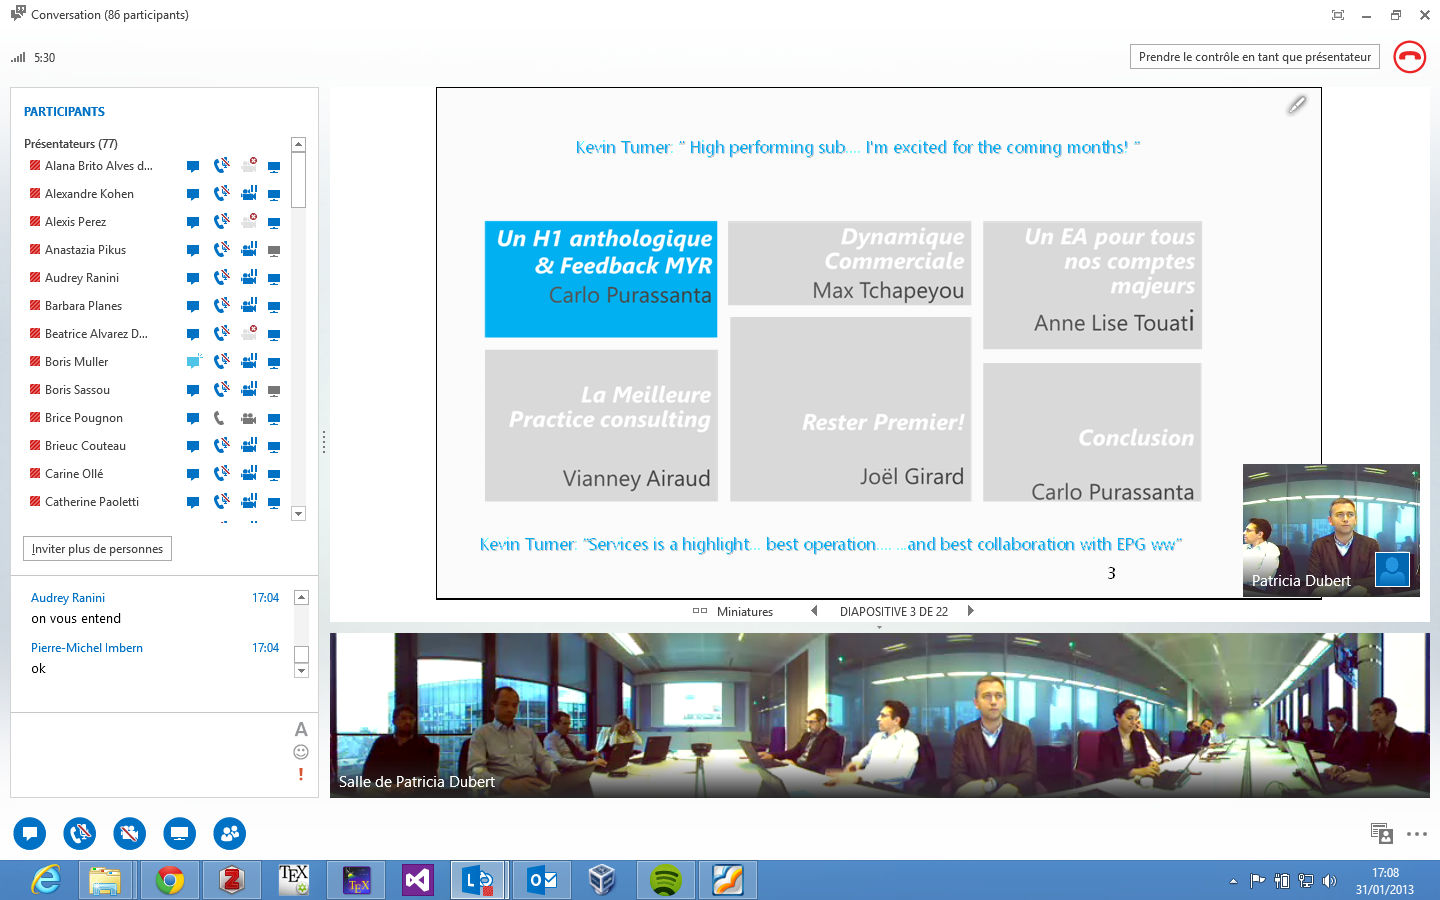
\includegraphics[width=0.8\textwidth]{Schemas/lync.pdf}
	\caption[Lync client connection]{Lync client connection (Adapted from figure 1.11 of \cite{winters_mastering_2012})}
	\label{fig:lync_poolfe}
\end{figure}

The figure \ref{fig:lync_poolfe} shows the steps required to connect a client to its home server in a front-end pool:
\begin{enumerate}
\item The client queries the DNS server to get the pool's IP
\item The DNS server returns all the IPs of the servers in the pool
\item The client connects to a random server from the pool
\item If this server is not the client's home server, it returns the name of the client's home server
\item The client queries the DNS server to get the home server's IP
\item The DNS server returns the client's home server's IP
\item The client connects to its home server
\end{enumerate}

\subsubsection{SharePoint Integration}
Lync Server can be integrated with SharePoint, which enables the skill search functionality, based on users' skills as specified on a user's SharePoint page. This allows SharePoint sites to display users' presence information based on the data provided by Lync servers, share users' pictures, or directly record and share meetings via SharePoint.

\subsubsection{Exchange Integration}
Lync Server can be integrated with Exchange, which adds unified messaging features, IM and presence to the OWA, and integration of contacts. 


\subsection{Architecture}
This section describes some key elements of a Lync architecture.

\subsubsection{Central Management Store (CMS)}

The Lync Central Management Store is a database holding the configuration information for the Lync topology. This database is replicated on all front-end and back-end servers of an enterprise pool. This data can be modified by the Topology Builder, the Lync Server Control Panel, and the Lync Server Management Shell. Access to this database is required for any change to the architecture of the solution. It is recommended to pay particular attention to the availability and backup of this database.


\subsubsection{Sites}

Lync sites define a region of the network containing Lync Server components in which the connectivity is good: the connection between computers of a site has a high speed and low latency. A Lync site can either be a central site, if it contains at least a front-end server (either a Standard edition server, or an enterprise pool), or a branch site, which depends on a central site to provide some Lync services to its users.

A branch site providing telephony services to its users can have a Survivable Branch Appliance (SBA) for sites under 1,000 users or a Survivable Branch Server (SBS) for sites between 1,000 and 5,000 users, which have the Lync Server Registrar and a Mediation server. 

Although their definitions are similar, Lync sites and AD sites do not need to correspond
\cite{microsoft_technet_sites_2012}.


\subsubsection{Policies}

The behavior of the Lync solution is configured by policies which are assigned to users or sites. The management of these policies is an important part of the design and the administration of a Lync solution. Some of these policies are:

\begin{description}
\item[Client policy] A client policy defines the behavior of the Lync client software, such as which features are available and some client settings. Until Lync server 2010, these settings were controlled via an AD Group Policy. This policy can only be assigned to users.

\item[Client version policy] This policy defines which client versions are allowed to log on to Lync Server and which are blocked. This policy can also force silent upgrades of the client, or redirect the user to an URL to download a new version. The Lync server checks the SIP headers to determine the client version, and compares it the client version policies applicable for the user. Client version policies can be applied at the global, site, service or per-user scope.

\item[Conferencing policy] Conferencing policies determine which features and capabilities can be used in a conference. Conferencing policies can be applied at the global, site, or per-user scope.
\end{description}

Therefore, to define the permissions and behavior of the solution for an user, multiple policies have to be combined. The precedence of policies (eg. a per-user policy overrides a global policy) has to be taken into account when designing the user profiles.


\subsubsection{Autodiscover}
The autodiscover features allows a client to connect to the Lync infrastructure given only the SIP address of the user. Combined with SSO, this allows the user to connect to Lync without any action.

The autodiscovery method to find the registrar server is based on DNS queries, using the domain name of the SIP address. The queries depend on the client used. For example, for an user with a SIP address of sip:user@domain, the following queries will be made:

\begin{description}

\item[Lync 2013]
\begin{itemize}
\item Host (A) record lyncdiscoverinternal.domain
\item Host (A) record lyncdiscover.domain
\item Service Locator Record (SRV) record \_sipinternaltls.\_tcp.domain
\item Service Locator Record (SRV) record \_sip.\_tls.domain
\item Host (A) record sipinternal.domain
\item Host (A) record sip.domain
\item Host (A) record sipexternal.domain
\end{itemize}

\item[Lync Mobile]
\begin{itemize}
\item Host (A) record lyncdiscoverinternal.domain
\item Host (A) record lyncdiscover.domain
\end{itemize}

\item[Lync 2010]
\begin{itemize}
\item Service Locator Record (SRV) record \_sipinternaltls.\_tcp.domain
\item Service Locator Record (SRV) record \_sip.\_tls.domain
\item Host (A) record sipinternal.domain
\item Host (A) record sip.domain
\item Host (A) record sipexternal.domain 
\end{itemize}

\end{description}



\subsubsection{Media bypass}
The media bypass feature allows the audio flux to transit directly to the PSTN gateway, instead of using a mediation server. This can improve the call quality by reducing the latency and reducing the loss (as there is less transcoding), particularly for users of a branch site without a mediation server, as the media flux would go to the datacenter and back to the branch site before reaching the branch site PSTN gateways.

The media bypass can enabled for the whole solution, or for specific sites. If media bypass is enabled, the communication between the Lync client and the gateway is established via the G.711 CODEC.


\subsubsection{Call routing}
Lync calls routing uses the following components\cite{microsoft_technet_dial_2012}:

\begin{description}
\item[Dialplan] A dialplan is made up of different normalization rules, which can manipulate phones numbers. Users dialplan normalizes the phone numbers dialed by the users into the E.164 format. A dialplan can be assigned to each PSTN gateway to manipulate the caller and called number for inbound calls. A normalization rule is composed on a regular expression to detect the number, and the replacement expression.

\item[Voice Policy] A voice policy can be assigned to users, site or organizations to determine the Enterprise Voice functionality available.

\item[Route] A route allows an outgoing to connect via a mediation server to a gateway. Each route can be associated to multiple trunks.

\item[PSTN Usage] A PSTN usage is use to link voice policies and routes. There can be a many-to-many relationship between voice policies and PSTN usage, and between PSTN usage and routes.

\item[Trunk configuration] Allows number manipulation on outgoing calls.

\end{description}

\begin{figure}[h!]
	\centering
	\includegraphics[width=1\textwidth, page=6]{Schemas/lync_routing.pdf}
	\caption[Lync 2013 voice routing]{Lync 2013 voice routing. From Microsoft TechEd Africa 2013}
	\label{fig:lync_routing}
\end{figure}




%\section{Cloud solutions}
%\subsection{Office 365}
%\subsection{Microsoft Azure}
%\subsection{On-premises or in the cloud?}



\chapter{Case Study}\label{chapter_case}

\paragraph{}
\textit{This chapters presents the 30 000 Lync seats and telephony deployment which was the main focus of this thesis. The various stages, technical choices, and difficulties of the project are detailed.}


\section{Project Overview}
\paragraph{}
This section gives an overview of the project.

\subsection{The Client}
	The client is a french group with 250,000 employees, which will be called "Contoso" in this report\footnote{This company has requested that their name not be made public.}.
	
\subsection{Context}
	Contoso planned to move one of their offices to a new site, called in this report "Campus", and wanted to take advantage of this move to introduce Lync as a new communications solution, first to the 1,250 Campus users, then to 2,000 nomadic users and 30,000 other users.

	By introducing a new UC solution, Contoso IT direction's goals were:
	\begin{itemize}
		\item Meet the new user needs
		\item Offer new services
		\item Assist Contoso in its development and transformation
		\item Reduce IT and telephony costs and risks
	\end{itemize}

		
\subsection{Specifications}
	Contoso had the following broad specifications for the solution:
	\begin{itemize}
		\item Telephony features allowing the new solution to replace a traditional telephony solution
		\item Provide videoconferencing features
		\item Integration with the existing IT, telephony, and videoconferencing environments
		\item High availability and site survavibility
		\item Available from Contoso's internal network, and from an external network, on computers, smartphones, and tablets
	\end{itemize}

\subsection{The Constraints}
	As the project had to be completed in less than six months, time was a major constraint in this implementation.
	Moreover, Microsoft was responsible for the integration of various vendors' equipment into the solution, which induced additional risks.

\subsection{Stages}
	The project was split into 5 stages, according to the V-Model\cite{schuppan_cmm-based_2000, sheffield_systemic_2005} :
	\begin{description}
		\item[Requirements and Architecture] During this phase, the client requirements are gathered, and the overall architecture and features of the solution are defined. The deliverables of this phase include a summary of the workshops conducted with the client, and a high level specification of the solution.
		\item[Design] The goal of this stage is the redaction and validation of the detailed design document, which explains in detail the technical requirements and implementation of the solution.
		\item[Implementation] This is the main step realizing the concrete goals of the project. Expected deliverables are the installed solution and installation guides.
		\item[Test] During this phase, the solution is tested to confirm that it is working as specified in the design document. 
		\item[Validation] This stage validates that the solution can be used in the production environment according to the client's needs and the original specification from the first stage.
	\end{description}
	The stages are successive, but multiple stages can be active at the same time.
	\begin{figure}[H]
		\centering
		\includegraphics[width=0.8\textwidth, page=3]{Schemas/design.pdf}
		\caption{The V-model stages}
		\label{fig:case_vmodel}
	\end{figure}
	The following subsection describe the various stages of the model.


\subsection{Personal involvement}
	During the Requirements and Architecture stage, I gathered the client's requirements in a series of workshops.
	During the Design stage, I studied the Lync core architecture and dimensioning of the system, as well as the fixed and wireless network requirements and prerequisites for Lync, and was responsible for the associated sections of the design document.
	During the Implementation stage, I built and documented the core Lync integration infrastructure, and assisted the Contoso team in building the production infrastructure. During the Testing and Validation stage, I designed the test plan, wrote scripts, tested and validated the solution. 
	During all stages, I was responsible of the project documentation and prerequisites checking. 
	Further details of these stages are given in the following sections.

\section{Requirements and Architecture workshops}

	\paragraph{}
	Most of the time during the Requirements and Analysis phase was devoted to a series of nine workshops. Each workshop focused on a specific topic and involved one or two Microsoft consultants, the client project owner, and some relevant technical specialists for half a day to a full day.

	The first six workshops were planned from the beginning, while the others were added as the need for more clarification of particular topics arose.


\subsection{Architecture and Dimensioning workshop}

	\paragraph{}
		This first workshop's goal was to gather additional information regarding the project scope, the concerned population, usage models, to determine the general infrastructure architecture, and to begin the process of dimensioning the implementation.

		In order to dimension the implementation, we used the data found in the Lync Server 2013 User Models\cite{microsoft_technet_lync_2013}, unless the client could provide more specific information about their current and expected usage, in which case we would use the client's data.

	\paragraph{}
		Contoso had several requirements for the Lync infrastructure:
		\begin{itemize}
		\item A Contoso datacenter should host the main Lync Server 2013 farm, and should provide Lync services to multiple sites.
		\item The Lync infrastructure had to be highly available (expected availability of at least 99\%).
		\item The interconnection with the company's telephony infrastructure must be secure, but not the interconnection with unified messaging and videoconferencing.
		\item A disaster recovery plan was not required.
		\item The campus site should have survivability (i.e., telephony services should operate even if the connection to the datacenter is unavailable).
		\end{itemize} 

	\paragraph{}
		The unified communications solutions had to be available from:
		\begin{itemize}
		\item A cable-connected computer in any of Contoso's sites,
		\item A WiFi-connected computer in WiFi enabled sites,
		\item A WiFi-connected Apple iPhone or Apple iPad,
		\item A computer outside Contoso's network, connected through a VPN,
		\item An iPhone or iPad outside Contoso's network, connected through a VPN,
		\item A Lync or IBM Sametime federated user.
		\end{itemize}


\subsection{Information Systems Impacts workshop}
	\paragraph{}
	This second workshop focused on the interactions between the proposed solution and the existing IT infrastructure. Major interactions were expected with AD, DNS, PKI, Echange, SQL, and support for Lync on a separate disk under the customer's choice of Windows OS.

	\paragraph{Active Directory}
	AD was the first requirement, as AD is the base upon which many of Microsoft's products are based, including Lync Server 2013 or Exchange Server 2013. 
	Contoso's AD has multiple domains and forests and Lync Server 2013 should be installed in the COMMON.CONTOSO.FR and \linebreak COMMON.INTEGRATION.CONTOSO.FR domains, in which the user accounts to be used for Lync are located.

	Due to the critical nature of the AD infrastructure for the organization, any modification to the AD architecture usually requires a long advance notice. The Lync Server 2013 requires a schema extension and a domain/forest preparation, which required a one-month notice at Contoso, so we had to initiate the process early.

	If user accounts in another domain need to be activated for Lync, another domain preparation will be required.

	\paragraph{DNS}
	Lync Server 2013 relies on DNS requests to locate service providers, so we needed entries added to the internal and external CONTOSO.FR zones.

	\paragraph{Public Key Infrastructure}
	A public key infrastructure (PKI) is also required by Lync Server 2013, so Contoso had to designate the PKI to be used for Lync. Both the integration and production environments use the same Opentrust\cite{_opentrust_????} PKI, but with different certification authorities (CAs).

	\paragraph{Exchange}
	Each user's SIP address will be the same as their email address, hence they will have the following structure: sip:firstname.lastname@contoso.fr

	Contoso uses a Exchange Server 2010 infrastructure, but with a PKI different from the PKI used for Lync Servers, therefore the Exchange infrastructure must be modified to use the same PKI.
	The Autodiscover and Exchange Web Services were not currently enabled and had to be enabled.

	\paragraph{Windows}
	Contoso asked for Lync servers to be installed on Windows Server 2008 R2, and on a volume not used by the operating system's files. The last point required a supportability check, which turned out to be positive.

	\paragraph{SQL}
	Although Microsoft recommended the use of Microsoft SQL Server 2012, Contoso chose to use Microsoft SQL Server 2008 R2, because:
	\begin{itemize}
	\item Although SQL Server 2012 deployment was on Contoso's roadmap, it was scheduled for a later time.
	\item The Contoso team's current proficiency with SQL Server 2012 was low, and there was not sufficient time for training.
	\item The project criticality was too high to increase risks by trying a new solution.
	\end{itemize}



\subsection{Video interconnection and Internet workshop}
	\paragraph{}
	The solution had to be interconnected with Contoso's existing videoconferencing solutions and to provide services to some users over the Internet. This workshop allowed Contoso to express their needs on these topics.

	\paragraph{Videoconferencing}
	Contoso had an existing Polycom-based videoconferencing solution which needed to be integrated with the Lync-based solution. Their features requirements were:
	\begin{itemize}
	\item Integrate the Lync address book in the videoconferencing address book
	\item Show HDX and VSX\footnote{Videoconferencing endpoints produced by Polycom} equipments as contacts in Lync
	\item Peer to peer communications with HDX/VSX, with and without RTVideo license
	\item Conferencing between Lync, HDX and VSX clients in a Lync conference
	\item Conferencing between Lync, HDX and VSX clients in a RMX\footnote{Equipement produced by Polycom to host conferences} virtual conference room
	\item Document sharing with HDX and VSX equipments.
	\end{itemize}

	\missingfigure{Polycom HDX/VSX}


	\paragraph{Internet Access}
	The following usage scenarios require Internet access:
	\begin{itemize}
		\item Remote users connecting to Lync from outside Contoso's network
		\item Federated users
		\item Mobile users
		\item Anonymous users
	\end{itemize}

	To enable the Internet acces features, two components are needed: load-balancing and reverse proxy.
	Load-balancing can be either DNS-based, or hardware-based. The reverse proxy component is provided by Contoso.


\subsection{Telephony workshop}
	Contoso's main requirements for the solution were related to telephony features, as the Lync-based solution had to provide the same features that were provided by the various existing telephony systems in the other offices of the company.
	Of these requirements, the most critical were:
	\begin{itemize}
		\item Ability to call contacts inside or outside the company
		\item Single phone number, and the ability to use only the Lync application/phone
		\item Conferencing
		\item Auto callback, call forwarding, put a call on hold, response groups
		\item Caller ID
		\item Delegates
		\item Emergency calls
		\item 6-digit numbers for internal calls
	\end{itemize}

	Initially 1,200 telephony-enabled user accounts will be used at the Campus site, and Campus users must be able to use telephony services even if the Lync datacenter is unavailable. Of all users, a total of 6,500 users will be enabled for Enterprise voice.

	The Lync infrastructure must be interconnected with Contoso's other PBX through a G.729 CODEC. The gateways must be highly available.

	The phones considered for Campus deployment are:
	\begin{itemize}
		\item An Aastra Lync Phone Edition
		\item Two SNOM phones for delegates scenarios
	\end{itemize}

	The dial plan to follow was provided by Contoso.


\subsection{Network workshop}

	Contoso has two wide area networks (WANs) that will be available from the Campus site:
	\paragraph{1. Sirius}
		\begin{itemize}
			\item Layer 3 WAN
			\item 20 Mbps
			\item Diffserv classes used: 
				\begin{itemize}
					\item Audio
					\item Video
					\item Data high priority
					\item Data critical
					\item Data best effort
				\end{itemize}
			\item Service Level Agreement (SLA) on the quality of service for the audio and video classes
			\item 30\% of the bandwidth can be used by Lync
		\end{itemize}

	\paragraph{2. Ethernet based WAN deployed across the company}
		\begin{itemize}
			\item Layer 2 WAN
			\item 2x100 Mbps, upgradable to 1 Gbps
			\item Before Campus, used only for data
			\item No SLA
		\end{itemize}
			
	
	Contoso currently uses QoS on both WANs, based on the DSCP headers of packets. The current values are DSCP46 for Voice and Signalling, and DSCP AF41 for Video -- 
	All Lync traffic must be tagged to use QoS.
	
	In all the other offices, Contoso has two distincts VLANs for voice and data traffic. However, all Lync clients (desktop software, phones, or mobile application) generate audio, video, and data traffic.
	
	Campus's WiFi architecture was in the process of being redesigned. The projected WiFi architecture was to use 4 Cisco controllers (providing routing and firewall functionnality), and multiple light access points (acting only as relays).

\subsection{Operation and Supervision workshop}
	\paragraph{}
		This workshop focused on determining how the solution would be maintained and monitored by Contoso's teams during regular operation.

	\paragraph{Supervision}
		Contoso already uses System Center - Operations Manager (SCOM), and has a dedicated team. The current infrastructure is based on SCOM 2007, and monitors 1000 nodes out of a total of 3000 nodes.

		The SCOM team requires personalized rules to filter some of the Lync alerts.

	\paragraph{Operation}
		The main tools for Lync's operation are Powershell and the Lync Server Control Panel.

		As Lync's operating model is very close to Exchange's, Contoso wants their Exchange administration team to administer the Lync solution. Contoso's Exchange administration has the following properties:
		\begin{itemize}
			\item The service is administered with Powershell scripts and the Exchange console
			\item SCOM is used for supervision
			\item Role-based access control (RBAC) is currently being deployed
			\item The main support team administers servers while local teams administer users
			\item Users are classified by OU and delegations to these OU are assigned to regional administrators
			\item There are 25 regions, each with multiple sites and a single regional administrator
			\item Dell's (formerly Quest Software) MessageStats solution is used for monitoring
		\end{itemize}

\subsection{Additional Workshops}
	\paragraph{}
		These shorter workwhops were not scheduled at the beginning of the phase and were added as more information became available or when new needs emerged from the previous workshops.
		
	\subsubsection{Lync Mobile workshop}
		This workshop took place after the public release of the Lync Mobile 2013 client and specifications to review the integration of this Lync client with the implementation and Contoso's needs.
	
	\subsubsection{Desktop workshop}
		This workshop provided additional information about the desktop configurations that will be used at the Campus site, as well as desktop issues such as deployment and configuration of the clients, antivirus and firewall properties, and QoS client configuration.
	
	
	\subsubsection{Music on Hold workshop}
		The music on hold feature needs an audio file to play when a call is put on hold. There are two possible locations for this file:
		\begin{description}
			\item[On each client's computer] This is Microsoft's recommendation. However, this solution requires that the file is placed and updated on each client computer.
			\item[On a central file share] This solution removes the need to manage the music on hold file on each of the client computers, but can use more bandwidth and may cause problems for users connected through an Edge server.
		\end{description}

\subsection{Decisions}
	\paragraph{}
		According to the business and technical needs expressed by Contoso during the series of workshops, the following decisions were taken:
		\begin{description}
			\item[Sizing] The solution must be able to support 30,000 users, with 1,250 users at Campus.
			\item[Domains] The domains names to be used are CONTOSO.FR and ADATUM.COM\footnote{placeholder name for another company} with CONTOSO.FR being the default SIP domain.
			\item[Client] As many of the computers on the Campus site will run Microsoft Windows XP, the client deployed will be the Lync 2010 client.
			\item[Deployment in two phases] Due to the time constraint and the complexity of the project and of Contoso IT infrastructure and organization, the Edge server portion of the project was removed from the first phase. It will be implemented in a second implementation phase.
			\item[Only two environments] Contoso's usual deployement process involves three environments, each managed by a different team: Design, Integration, and Production. Due to the limited time available, only the Integration and Production environments will be involved for this project.
			\item[Single Datacenter] All Lync servers will be hosted in a single Contoso datacenter, and branch sites will connect to the datacenter, with a survavibility solution in case the connection to the datacenter is lost.
			\item[Redundancy] To ensure high availability with a goal of 99\% availability, all the components in the solution must have an n+1 redundancy. This includes the Lync servers, telephony gateways, reverse proxy and load balancing solutions.
			\item[Telephony] Lync should be the primary telephony solution for 1200 users at Campus. Users should use their local PSTN access for external calls. Lync should be interconnected with Contoso's telephony environment via the G.729 codec.
			\item[Security] To ensure the confidentiality of data and the integrity of the service, all traffic must be encrypted, and Lync Director servers must be used.
			\item[WAN usage] Due to the limited bandwidth available on SIRIUS, the Ethernet MAN is preferable for Lync data -- if the creation of priority classes and an operator SLA can be obtained.
			\item[New SCOM 2012 infrastructure] A new SCOM 2012 infrastructure is being deployed by Contoso and will be used for Lync.
		\end{description}


\section{Design}
\paragraph{}
The redaction of the Detailed Design Document was the main task of the design stage. This 300-page document explains the design choices and specifications.

This section provides an overview of the design of the final implementation, as specified in the Detailed Design Document.

\subsection{Prerequisites}
This section lists the requirements that had to be met by Contoso's infrastructure \textit{before} the implementation's construction could begin.

	\subsubsection{Active Directory}
		\begin{itemize}
			\item The forest functional level of the CONTOSO.FR forest must be Windows Server 2003 native.
			\item The domain functional level of the COMMON.CONTOSO.FR domain must be Windows Server 2003 native.
			\item There must be at least one AD DC which is a Global Catalog for the COMMON.CONTOSO.FR domain.
			\item The forest must be prepared for Lync 2013.
			\item An account with Domain Admin rights is required for deployment.
			\item A member of the RTCUniversalServerAdmins group is required for deployment.
		\end{itemize}
		
	\subsubsection{DNS}
		\begin{itemize}
			\item A, SRV and CNAME entries can be added to the DNS zones
			\item DNS zones CONTOSO.FR and ADATUM.COM must be configured in split-domain.
			\item The Lync infrastructe and internal clients must be able to resolve the following internal DNS zones: CONTOSO.FR, ADATUM.COM, and COMMON.CONTOSO.FR
			\item The Lync infrastructure in DMZ must be able to resolve external DNS zones CONTOSO.FR and ADATUM.COM
			\item External components accessing Lync services must be able to resolve the CONTOSO.FR and ADATUM.COM external zones.
		\end{itemize}
		
	\subsubsection{PKI and certificates}
		To allow Lync traffic to use TLS and MTLS connections, the Lync infrastructure requires X.509 certificates.		
		
		
\todo{Network requirements}


\subsection{Architecture}

	\subsubsection{Lync}
	Only one Lync site will be created for this implementation, called "Datacenter". A remote site "Campus" will also be created.
	
	Two SIP domains will be configured in production: CONTOSO.FR and ADATUM.COM, with the CONTOSO.FR domain configured as the default SIP domain.
	
	The dialin, meet, and admin simple URLs will be used in this implementation. To allow the addition of new SIP domains while limiting the number of new certificates needed, the meet and dialin URLs have been chosen as follows: https://lync.contoso.fr/contoso/meet https://lync.contoso.fr/adatum/meet and \linebreak https://lync.contoso.fr/dialin .
	The administration URL will be \linebreak https://lyncadmin.common.contoso.fr
	
	
	\subsubsection{DNS}
	Lync client connection should be automatic, which means that after the user has logged into his Windows session, no configuration or password are required for Lync to connect. As Lync 2010 and 2013 clients will be used, the following DNS records will all have to be created:
	\begin{table}[H]
	\centering
	\begin{tabular}{c|l}
		Record Type & Value \\ \hline 
		A & lyncdiscoverinternal.contoso.fr \\
		A & lyncdiscoverinternal.adatum.com \\
		A & lyncdiscover.contoso.fr \\
		A & lyncdiscover.adatum.com \\
		SRV & \_sipinternaltls.\_tcp.contoso.fr \\
		SRV & \_sipinternaltls.\_tcp.adatum.com \\
		SRV & \_sip.\_tls.contoso.fr \\
		SRV & \_sip.\_tls.adatum.com \\
		A & sipinternal.contoso.fr \\
		A & sipinternal.adatum.com \\
		A & sip.contoso.fr \\ 
		A & sip.adatum.com
	\end{tabular}
	\caption{\label{tab:case_dns} DNS records}
	\end{table}

	
	\subsubsection{PKI}
	This section lists the certificate requirements for the Lync solution. To limit the number of subject alternative name (SAN) by certificate, Contoso wishes that each certificate be deployed on only one server, if possible.
	
	\missingfigure{Certificate table}
	
	\subsubsection{Strategies}
	
		This section lists various configuration choices that have to be implemented in Contoso's Lync infrastructure to enable the desired behavior.
		
		\paragraph{Monitoring} All CDR and QoE records will be kept for 180 days.
		
		\paragraph{QoS} To enable QoS tagging of Lync traffic, the client and server ports used by Lync will be configured as follows:

		\begin{table}[H]
		\centering
		\begin{tabular}{lllc}
			Endpoint & Type & Ports & DSCP  \\ \hline 
			Front End servers & Audio & 30000 - 36999 & 46 \\
			Front End servers & Video & 37000 - 37999 & 20 \\
			Front End servers & Application sharing & 38000 - 38999 & 16 \\
			Exchange UM & Audio & 30000 - 36999 & 46 \\
			Gateways & Audio & 30000 - 33999 & 46 \\
			Clients & Audio & 30000 - 30039 & 46 \\
			Clients & Video & 37000 - 37039 & 20 \\
			Clients & Application sharing & 38000 - 38039 & 16 \\
			Clients & File transfer & 39000 - 39039 & - \\
			SNOM phones & Audio & 30000 - 30039 & 46 \\
		\end{tabular}
		\caption{\label{tab:case_qos} QoS configuration}
		\end{table}
	
	
	\subsubsection{Lync/Exchange integration}
	The following Lync 2010 client features depend on the Lync/Exchange integration:
	\begin{itemize}
		\item Contact information
		\item Calendar information
		\item Conversation history
		\item Missed conversations
		\item Missed calls
		\item Voice Mail Playback
	\end{itemize}


\subsubsection{High Availability}
This table describes the behavior of the solution when one or more of the components fail or lose connectivity:

\begin{table}[H]
		\centering
		\begin{tabularx}{\textwidth}{lcX}
			Component & \# nodes & Impact  \\ \hline 
			Front End & 1 & No Impact \\
			Front End & 2-3 & Performance might be reduced \\
			Front End & 4-7 & All Lync services unavailable, except for local survivability \\
			Edge & 1 & No impact \\
			Edge & 2 & Edge features unavailable \\
			OWA & 1 & No impact \\
			OWA & 2 & Performance might be reduced \\
			OWA & 3 & No presentation sharing \\
			Back End & 1 &  No impact if witness is operational \newline Else, see below\\
			Back End & 2 & User are switched to resiliency mode \\
			Director & 1 & No impact \\
			Director & 2 & No external login \\
			DFS & - & No change can be made to the infrastructure \\
			Reverse Proxy & - & No Lync mobile clients support \newline No external web services \\
		\end{tabularx}
		\caption{\label{tab:case_ha} Availability table}
		\end{table}



\subsubsection{Load Balancing}
High availability requires load balancing for some components. Load balancing allows the distribution of requests among the available nodes.

There are two types of load balancing used for the Lync infrastructure: DNS load balancing, and using a Brocade Hardware Load Balancer (HLB).

The Brocade HLB is used to balance the HTTP/HTTPS traffic to the Front End pool, the Directors, and the Office Web Apps farm, while other traffic uses DNS load balancing.



\subsubsection{External usage}

There are three external usage scenarios possible:
\begin{description}
	\item[Case 1] Users are directly connected to the Internet.
	\item[Case 2] Users are connected through a VPN tunnel, and all traffic goes through the VPN tunnel.
	\item[Case 3] Users are connected through a VPN tunnel, but the solution allows split tunneling for Lync traffic.
\end{description}
Case 1 is Microsoft's recommended use case. Case 2 is not supported, as the VPN equipment can degrade the overall call experience. Case 3 is supported, but requires additional work on the VPN infrastructure.

Clients with a mobile device, such as an Apple iPhone or Apple iPad, use the same infrastructure with different access mechanisms, as these clients use the Lync 2013 Unified Communications Web API (UCWA) component which was introduced with Lync 2013 Cumulative Update 1, and installed on the front end server pool.






\subsection{Infrastructure}
	The following sections give high level descriptions of the implementation's infrastructure.

	\subsubsection{Internal infrastructure}
	The internal infrastructure is comprised of all of the servers and equipments connected to Contoso's internal network.
	Therefore, it is made up of:
	\begin{description}
		\item[Lync clients] Desktops, laptops, tablets, phones, or smartphones, the client devices are connected via ethernet or WiFi and allow users to access Lync services.
		
		\item[7-server Lync Front-End pool, with collocated mediation server] In this implementation, the Front-End pool has the following tasks:
			\begin{itemize}
				\item SIP server: SIP registrar, SIP  session initiation and management,  and presence information;
				\item Audio and video conference room; and
				\item Mediation server with a PSTN gateway.
			\end{itemize}
		According to the company's existing usage data and Microsoft's recommendations, each server can handle 6,660 concurrent users, hence 5 servers are required for 30,000 concurrent users. An extra server is added to handle the additional traffic caused by mobile usage, and another server was added  to meet the high availability requirement. Therefore, seven servers are required. Each of these server meets the following system requirements:
		\begin{itemize}
			\item 2 x 6-core processor (12 cores)  2,33 GHz
			\item 32GB RAM
			\item System and Lync binaries disk: 2 x 300GB 10K RPM SAS - RAID1
			\item Lync local database disk: 6 x 300GB 10K RPM SAS - RAID10
			\item 1 Gbps network link
		\end{itemize}
		
		
		\item[3 SQL Servers] Two servers are Back-End servers in a mirroring configuration and host the Lync databases. The third server is a witness server used for automatic failover in case of failure of one of the Back-End servers.
		Each back end server must meet these system requirements:
		\begin{itemize}
			\item 2x6-core processor (12 cores)  2,33 GHz
			\item 32GB RAM
			\item System and SQL server binaries disk: 2 x 300GB 10K RPM SAS - RAID1
			\item Lync database disk: 6 x 300GB 10K RPM SAS - RAID10
			\item Lync monitoring database disk: 6 x 300GB 10K RPM SAS - RAID10
			\item 1 Gbps network link
		\end{itemize}
		The SQL witness must meet these system requirements:
		\begin{itemize}
			\item 2x4-core processor (12 cores)  2,33 GHz
			\item 8GB RAM
			\item System and SQL Express binaries disk: 2 x 146GB 7.2K RPM SAS - RAID1
			\item 1 Gbps network link
		\end{itemize}
		
		
		\item[3-server Office Web App pool] An Office Web App server is required for displaying shared PowerPoint presentations during conferences.
		According to the usage data and Microsoft recommendations, each server can handle 20.000 concurrent users, which means that 2 servers are required for 30.000 concurrent users. An extra server has to be added to meet the high availability requirement. Therefore, 3 servers are required, with the following system requirements:
		\begin{itemize}
			\item 2x8-core processor (16 cores)  2,33 GHz
			\item 16GB RAM
			\item System and Office Web App binaries disk: 2 x 300GB 10K RPM SAS - RAID1
			\item 1 Gbps network link
		\end{itemize}
		
		\item[A highly available DFS share] A Contoso file sharing infrastructure, used for Lync data storage. 200GB must be available for Lync Server 2013 on this file share.
		
		\item[A Watecher Node] This server monitors the solution's components and reports their status to the SCOM supervision infrastructure. The SQL Server Reporting Services (SSRS) will also be installed on this server.
		The server must meet these system requirements:
		\begin{itemize}
			\item 4-core processor (4 cores) 2,33 GHz
			\item 8GB RAM
			\item System disk, with a 100Gb partition for SSRS databases and logs: 2 x 300GB 10K RPM SAS - RAID1
			\item 1 Gbps network link
		\end{itemize}
		
		\item[1 SNOM provisionning server] This server is required for automatic provisionning of SNOM phones.
		Its system requirements are:
		\begin{itemize}
			\item 4-core processor (4 cores) 2,33 GHz
			\item 4GB RAM
			\item System disk: 2 x 146GB 7.2K RPM SAS - RAID1
			\item 1 Gbps network link
		\end{itemize}
		
		\item[4 SBC Sonus UX2000 gateways] 2 in the datacenter, 2 at Campus, they respectively provide interconnection with the SIRIUS WAN and Campus's PSTN access.
		Datacenter gateway requirements:
		\begin{itemize}
			\item 1 UX2000-600 (UX2000 with 6 high capacity DSP, allowing 600 concurrent calls)
			\item 1 UX2000-T1E1-2 (A two-card E1 module)
			\item 5 UX-SIP-25 (5x25 = 125 SIP lisenses)
		\end{itemize}
		Campus gateway requirements:
		\begin{itemize}
			\item 1 UX2000-200 (UX2000 with 2 high capacity DSP, allowing 200 concurrent calls)
			\item 1 UX2000-T1E1-2 (A two-card E1 module)
			\item 2 UX-SIP-25 (2x25 = 50 SIP lisenses)
		\end{itemize}
		
		
		\item[A Survivable Branch Server] This server allows basic telephony features to remain accessible at the branch site if the Lync infrastructure at the datacenter becomes unreachable.
		Its system requirements are:
		\begin{itemize}
			\item 2x6-core processor (12 cores) 2,33 GHz
			\item 32GB RAM
			\item System and Lync binaries disk: 2 x 300GB 10K RPM SAS - RAID1
			\item Lync local databases disk: 2 x 300GB 10K RPM SAS - RAID1
			\item 1 Gbps network link
		\end{itemize}
		
		
		\item[2-server Lync Director pool] This server pools is responsible for authentication and redirection of users to their home front end server.
		Each server of the pool must meet these system requirements:
		\begin{itemize}
			\item 2x4-core processor (8 cores) 2,33 GHz
			\item 16GB RAM
			\item System and Lync binaries disk: 2 x 300GB 10K RPM SAS - RAID1
			\item Lync local database disk: 2 x 300GB 10K RPM SAS - RAID1
			\item 1 Gbps network link
		\end{itemize}
		
	\end{description}

\begin{figure}[H]
	\centering
	\includegraphics[width=0.9\textwidth]{Schemas/design.pdf}
	\caption{Internal infrastructure}
	\label{fig:case_internal}
\end{figure}
\missingfigure{Campus Infrastructure schema}


	\subsubsection{External infrastructure}
	The external infrastructure allows communications with networks other than Contoso's, such as the Internet, or the PSTN.
	The external infrastructure is made up of:
	\begin{description}
		\item[2-server Lync Edge pool] This pool handles all non-web traffic, such as voice, video, and sip, from and to external users and federated edge servers. This pool is placed in the DMZ. Each server can handle 12.000 concurrent connections, so only one server and one server for high availability are required, with the following system requirements:
		\begin{itemize}
			\item 2x4-core processor (8 cores) 2,33 GHz
			\item 16GB RAM
			\item System and Lync binaries disk: 2 x 300GB 10K RPM SAS - RAID1
			\item Lync local databases disk: 2 x 300GB 10K RPM SAS - RAID1
			\item 2x1 Gbps network link (one interface connected to the internal network, one interface connected to the Internet)
		\end{itemize}
		
		\item[2 Reverse-proxy servers] These servers relay https traffic from mobile and external users. These servers are placed in the DMZ
	\end{description}
	\begin{figure}[H]
		\centering
		\includegraphics[width=0.9\textwidth, page=2]{Schemas/design.pdf}
		\caption{External infrastructure}
		\label{fig:case_extternal}
	\end{figure}

	\subsubsection{System requirements}
	\missingfigure{sysreq table (and remove from above)}






\subsection{Telephony}

This section describes the design of the telephony components of this implementation.

\subsubsection{Overall Architecture}
	The telephony architecture is based on the main datacenter, and the campus site.

	\paragraph{Datacenter}
	The datacenter hosts the mediation pool, which is collocated with the front end pool, and interconnects the Lync infrastructure with the SIRIUS network via the SONUS gateways and a SBC Acme Packet cluster, and with the PSTN via the SONUS gateways.
	
	Contoso's ToIP network has some specificities requiring special consideration, for example only the G.729 ALaw codec is supported, as some equipments are incompatible with the G.729 BLaw codec. Moreover, some Aastra PBX only support the G.711 codec. This influenced the choice of the Sonus gateways, and their configuration.
	

	\paragraph{Campus}
	Due to the requirements for the Campus site, the Microsoft recommendations and Contoso's preference, it was decided to install an SBS with gateways at the Campus site.
	
	To increase call quality, media bypass should be activated for the Campus site.


\subsubsection{Interconnection with the ToIP network}
	Two different scenarios were available for the interconnection with Contoso's ToIP network, differing in the location of the transcoding, the bandwidth used, call quality, ease of configuration and cost.
	\begin{description}
		\item[Interconnection via the local gateways] 
			In this scenario, the gateways at the Campus site connect directly to the SBC Acme Packet cluster.
			\missingfigure{local gateways schema}
			\missingfigure{advantages/drawbacks table}
		\item[Interconnection via the central gateways] 
			In this scenario, the gateways at the datacenter connect to the SBC Acme Packet cluster.
			\missingfigure{central gateways schema}
			\missingfigure{advantages/drawbacks table}
	\end{description}
	
	As voice quality is an essential factor for the Campus site, and the RTT is not guaranteed to be under 25ms, the interconnection via the local gateways was chosen for this implementation.
	
	
\subsubsection{Interconnection with the PSTN}

	The solution is interconnected with the PSTN from the datacenter and the Campus site, with each access serving different purposes.
	
	\paragraph{Datacenter interconnection with the PSTN}
	This access serves 2 main purposes:
	\begin{itemize}
		\item access point for PSTN conference attendees.
		\item acces to the PSTN for users at a site without PSTN access
	\end{itemize}
	
	Between the PSTN and the front end pool, the G.711 codec is used, while between the front end pool and users from a site without PSTN access, the codec used can be either G.711 or RTAudio Narrowband if the RTT is above 25ms.
	\missingfigure{Datacenter interconnection with the PSTN}
		
	
	\paragraph{Campus interconnection with the PSTN}
	This access serves 2 main purposes:
	\begin{itemize}
		\item access point for PSTN conference attendees.
		\item acces to the PSTN for users at a site without PSTN access
	\end{itemize}
		
	\missingfigure{Campus interconnection with the PSTN}

	
\subsubsection{Sizing of the Sonus gateways}
	To appropriate sizing of the Sonus gateways was determined using usage provided by Contoso. According to this data, the relevant values are: 
	\begin{itemize}
		\item 0.014 Erlang/user for PSTN calls
		\item 0.025 Erlang/user for inter-site calls from the Datacenter
		\item 0.03 Erlang/user for inter-site calls from branch sites
	\end{itemize}
	These values are lower than Microsoft's recommendation, but will be used for the sizing, as they reflect Contoso's usage. However, in case of increased usage, it will be possible to increase the capacity of the gateways easily.
	
	For determining the number of lines required, we used the Erlang-B formula, with a maximum grade of service of 0.01 (When the usage is maximal, less than 1\% of incoming calls can be blocked due to insufficient lines)\cite{qiao_robust_1998}.
	
	
	\paragraph{Datacenter}
	Only 1,500 users will use the datacenter's gateways, the other 5,000 users will use their local site PSTN infrastructure for PSTN calls. The 1,500 users using the datacenter's gateways will use $1500*0.025 = 37.5 E$ for calling other sites which requires 50 SIP circuits, as well as $1500*0.014 = 21 E$ for PSTN calls, which requires 31 PSTN circuits.
	
	The datacenter will be used by 6,500 users enabled for Enterprise Voice. The datacenter's gateways will handle PSTN traffic for audio conferences. Contoso states that conference calls amounts to a third of all regular calls, therefore audio conference will use $6500 * 0.025 * 1/3 = 54 E$ which requires 68 SIP circuits, as well as 10 PSTN circuits.
	
	Each gateway will use 118 SIP circuits, which requires 5 SIP modules (25 SIP licenses each), and 41 PSTN circuits, which requires 2 E1 cards (included with the UX2000-600 gateways).
	
	\paragraph{Campus}
	The 1,250 Campus users enabled for Enterprise Voice will use $1250 * 0.014 = 17.5$ Erlang for PSTN calls and $1250 * 0.03 = 37.5$ Erlang for inter-site calls, which will require 27 PSTN circuits, which requires 2 SIP modules (25 SIP licenses each) and 1 two-E1-card module (included with the UX2000-200 gateways).
	

\subsubsection{Mediation server role}
If the Mediation server role is co-located on the Front End pool, each server is able to handle 150 concurrent calls. As there are 7 servers in the Front End pool, up to 1050 concurrent calls can be handled, which is a lot more than the number of available circuits on the datacenter gateways.

At the Campus site, the media bypass feature is activated, therefore the SBS will only be used during signalization, and the number of concurrent calls will be limited by the gateways.

The Lync infrastructure will be configured to use Mediation server redundancy so that the datacenter's Mediation servers will be used for Campus users' call signaling if the SBS is disabled.

\subsubsection{Dialing and number manipulation}
	\paragraph{Phone numbers format}
	Microsoft recommends the use of numbers formatted according to the E.164 standard. Therefore, Lync users will have a phone number of the following form: +33ZABPQMCDU;ext=DDSCDU where
	\begin{itemize}
		\item DD is the site identifier (for example 38 for Campus)
		\item S is a subsite identifier (0 or 1 for Campus)
		\item CDU is the user line identifier
	\end{itemize}
	
	All contoso users have a 6 digits internal number. However, for users outside campus, there is not always a logical relation between their internal and external number. For example an user with the internal number 393202 can have the external number +33123451234 instead of +33123453202.
	
	Because of this, it is impossible to create generic normalization rules.
	
	
	\paragraph{Types of traffic}
	There are three types of telephony traffic possible, each involves a different number manipulation process.
	\missingfigure{Types of telephony traffic}
	
	\paragraph{PSTN to Lync}
	\begin{description}
		\item[Called number] Usually, the operator provides the last 4 digits of the called number. The Lync front end server translates this number to a E.164 number according to the dialplan corresponding to the gateway.
		\item[Caller number] Can be either a national number (usually 9 digits), an international number (of variable length) or an anonymous number. If the number is national or international, the getway translates it into an E.164 number.
	\end{description}
	\missingfigure{PSTN to Lync}

	\paragraph{Lync to PSTN}
	\begin{description}
		\item[Called number] The Lync server does the translation before sending the number to the gateway.
		\item[Caller number] The gateway translates the caller number from E.164 to a 9-digit number.
	\end{description}
	\missingfigure{Lync to PSTN}

	\paragraph{ToIP to Lync}
	\begin{description}
		\item[Called number] The SBC returns a 6-digit number. The Lync server translates the number to a E.164 number according to the datacenter's dialplan (as only the datacenter's gateways are connected to the ToIP network).
		\item[Caller number] The SBC returns a 6-digit number. There is no manipulation on this number. However this prevents the resolution of the caller id for missed calls.
	\end{description}
	\missingfigure{ToIP to Lync}

	\paragraph{Lync to ToIP}
	\begin{description}
		\item[Called number] Most internal numbers are 3 or 6 digits numbers, but some have variable length. Therefore, the +0000 prefix has been chosen to identify internal number. This prefix is added by the Lync client. The Lync server removes and normalizes the number into a E.164 number, and the gateway translates the number into a 6 digit number.
		\item[Caller number] The Lync client sends a E.164 number, which is translated into a 6 digit number by the gateway.
	\end{description}
	\missingfigure{Lync to ToIP}
	

\section{Deployment}

\paragraph{}
This section describes the deployement of the implementation, and some of the challenges encountered.

\subsection{Construction}
	The previously detailled implementation was deployed on Contoso's architecture in two steps: 
	\begin{description}
		\item[Integration] First Microsoft consultants setup the solution in the integration environnement, and checked that the solution behaved as expected. Based on this implementation, some modifications to the design were made, and construction guides detailling the construction process were redacted. This purpose of this environment is to be able to make sure the solution is designed correctly, that the integration between the solution and others is operational, and that the installation process does not impact other services. Every new solution or update to a solution is applied in the integration environment before going into production. 
		
		\item[Production] Contoso's teams then deployed the solution in the production environment according to the construction guides. This allowed the Contoso team to familiarized themselves with the solution and ask specific questions about the design.
	\end{description}


\subsection{Testing}
	To ensure the solution behaved as expected and no mistake was during the design or construction phases, testing was an important part of the project. Different kinds of tests were realized, for different purposes:
	
	\begin{description}
		\item[Built-in tests] Some tests are part of the installation scripts, and are run automatically during construction to validate that the prerequisite for installation are met, or that the previous step was successful. The installation of the Lync Server 2013 binaries includes many of these tests, to check that the AD domain and forest are correctly prepared or that all Lync components are correctly installed.
		
		\item[Unit tests] Unit tests are run to validate that a particular component of the solution taken independently functions as intended. These tests include scripts running Lync synthetic tests cmdlets or checking the status or response of a component.
		 
		\item[Integration tests] These tests are run to validate that the interactions between different components or solutions are correct. Integration testing was crucial to validate the telephony features and identify and fix problems early.
		
		\item[Functional tests] A functional test follows a user scenario to validate that the user experience is good. An example of a functional test would be creating a conference between Lync and HDX users, add video, share a document, invite a participant, then view the recording.
	\end{description}

	These tests were run at varying points and intervals during the construction:
	\begin{description}
		\item[During construction] Some tests (automatic or manual) were run during the construction of the solution, between steps, to ensure that the prerequisites were met, prevent human error or identify differences between environments.
		
		\item[Regularly] Some tests are run at regular interval (from 1 day to 1 week) to detect problems early, and ensure non regression during construction.
		
		\item[During the test phase] For a construction phase (integration or production environment) to be validated, the solution has to pass all required tests at the same time. If some tests fail, corrections are made, and all tests are run again, until the results are acceptable.
	\end{description}

\subsection{Usage}
 The introduction of Lync to the new users was done in multiple steps. First, the solution was presented to users in internal events, showcasing some of the features and benefits of Lync, so that users can be more familiar with the solution in order to accept the change better.
 
 In a second phase, some users were given access to Lync, first on a proof-of-concept infrastructure, then on the real infrastructure. Users were added in three successive groups, for a total of more than 500 users. The goal of this phase was to begin to test how Lync would be used and received by the users, as well as to train some users (the first users selected were in IT teams, and will have to provide support or administer the production solution) and increase adoption. This phase showed that Lync was well received by users, and more than 80\% of users used Lync regularly during the test. However, some obstacles to Lync adoption were reported: 
\begin{itemize}
	\item A regular telephony solution was maintained during the test (for the first 2 waves)
	\item Not all users were using Lync (the best Lync usage was obtained when full teams were involved in the test)
	\item Some technical problems and missing features were reported on the proof-of-concept environment
	\item The training for test users was minimal and users were frustrated not to be able to perform some actions.
\end{itemize}

In the third phase, all future Campus users were given detailed FAQ sheets and procedures for the most common tasks, such as changing the profile picture, forwarding a call, or organizing and joining a conference. Users and administrators were also given specific training depending on their role, to ensure that users will know how to use the solution and avoid getting stuck on simple tasks when they move to Campus.


\subsection{Difficulties}
	Almost all the problems encountered during this project has one of the following root causes:
	\begin{description}
		\item[Multiple teams involved] As unified communications spans many domains, multiple teams had to work together on this project, belonging to different departments, such as IT, telephony or videoconferencing. At Contoso, these teams are not used to working together, are located 400km apart and do not all have the same priorities and schedules. This caused a lot of planning problems, as all teams depended on others to advance, so a lot of time was spent waiting or coordinating teams.
		
		It is worth remarking that a common problem with Lync deployments, which was not encountered at Contoso as the solution did not replace any existing service, is the reluctance of one or more of the involved teams, as Lync can move some of their responsibilities to other teams (usually telephony responsibilities going to IT).
		
		\item[Different design philosophy] A recurrent problem was the difference between Lync's design philosophy and choices and the habits of users used to using classic telephony systems for years. Unlike telephony systems, Lync is design is "user-centric", so Lync is designed around the idea that users try to reach an user, and not a number. Therefore, some telephony features are less relevant in Lync, and were not included. Some of these features were introduced in the Lync Cumulative update 1 (such as call pickup) due to feedback from the early adoption program, but others features needed third party software (such as advanced delegation support).
		
		Moreover, some situations encountered by Contoso were not included in Lync's design, such as their sites and regions layout, which might cause performance problems due to the complexity of the resulting dialplans and routing tables.
		
		Some of these problems can be solved through user training, and the creation of new habits, but others will require modifications to the Lync client and server software.
		
		\item[Integration with components from other vendors] The implementation had to interact with different systems, many of those from other vendors. Therefore there were some problems during construction, either because we depended on the vendor's support teams to install or configure equipment, or because of incompatibilities between Lync and the other vendor's equipment. For example, we had to wait for Polycom's updates to connect their products to the implementation, and the direct connection between Lync and a VSX still requires a update that has not yet been released.
	\end{description}

	
%\section{Conclusion}The solution has been delivered on schedule, and is currently the main communication solution at the Campus site. Other Contoso sites will soon be able to use this same solution.Although some features originally planned had to be removed due to the time constraint, the core features required by Contoso are operational, and a newThe solution has been well accepted by the users



\chapter{Conclusions and Future Work}

\section{Telephony with Lync 2013}

This master's thesis project demonstrated that Lync 2013 can be en effective solution for multiple purposes, including a complete telephony replacement. 

This project also helped providing data and feedback about Lync server 2013. This led to two upgrade requests to the product development team (improvments to the call deleguates features and to the call routing) and some of the data was used to redact the reference documents for deploying Lync Server 2013.

The project also showed that although technical problems can arise during the construction of an unified communications solutions based on Lync, most problems, and the most critical problems are organizational problems, or problems that can be resolved through the analysis of the users' needs and user training.


\section{Future Work}

\subsection{Contoso's implementation}
This implementation can still be improved, by adding the edge features that were cut due to the time constraint, which will allow external connections and federations scenarios. It's also possible to consider the addition of the other remote sites, and their particular needs. Another aspect that was left out of this project is a complete backup/restore, disaster recovery and PSTN access redudancy plan.

\subsection{Lync and Unified Communications}
Some aspects of Lync were not studied in this project, and might be of interest, such as the integration of the Lync 2013 client, or the use of Lync as a platform for more complex applications, such as a call-center, with the use of the Lync APIs.

A more in-depth study of Lync's network usage, including QoS and CAC impact would be helpful in determing precisely the right network sizing for future implementations.

\section{Reflections}
This master's thesis project is the design and construction of an unified communication solution, used for instant messaging, conferencing and telephony. Unified communications solutions can have a variety of positive consequences for companies, but other effects may require further reflection or attention when planning an unified communications solution.

One the most common cause of concern for employees when an unified communications solution is introduced in the workplace is due to the presence indicator, which is a central part of all UC solutions. Employees fear that this feature can be used to track their worktime, their activity, or their communications. Moreover, if UC solutions can help remote workers, it can also lead to the employees being asked to stay connected and available for work all the time, even outside the workplace. These practices are usually controlled by legislation.
%\todo{In France?} the privacy of electronic communications for employees, including UC solutions communications, is guaranteed by the law, as well as the work duration and conditions.

UC solutions can also pose a threat to the safety of people if not planned correctly, as UC solutions can be used for calling emergency number, but do not automatically provide the same services, such as location information. There are a variety of solutions to this problem, from configuring the UC solution to include location information to disabling emergency calling on UC phones and instructing users to call from an emergency phone, or cell phone.

\bibliographystyle{myIEEEtran}
\bibliography{IEEEabrv,biblio,rfc}
\addcontentsline{toc}{chapter}{References}


%\backmatter

\end{document}
